\documentclass[conference]{IEEEtran}

\usepackage[utf8]{inputenc}
\usepackage[T1]{fontenc}
\usepackage{amsmath}
\usepackage{booktabs}
\usepackage{multirow}
\usepackage{array}
\usepackage{url}
\usepackage{cite}
\usepackage{stfloats}
\usepackage{graphicx}
\usepackage{hyperref}

\hypersetup{
    colorlinks=true,
    linkcolor=black,
    citecolor=black,
    urlcolor=black
}

\graphicspath{{../rl_notebook_figures/}{rl_notebook_figures/}{KDS/Sürüden_keep_cull/reports/rl_notebook_figures/}}

\renewcommand\IEEEkeywordsname{Anahtar Kelimeler}

\title{Süt Sığırcılığında İnek Bazlı Elde Tutma/Sürüden Çıkarma Kararları için Hibrit Denetimli Risk ve Model Tabanlı Pekiştirmeli Öğrenme Prototipi}

\author{
\IEEEauthorblockN{Artun Kara}
\IEEEauthorblockA{
Kocaeli Üniversitesi\\
Kocaeli, Türkiye\\
artunankara@gmail.com}
}

\begin{document}
\maketitle

\begin{abstract}
Süt sığırcılığı işletmelerinde inek bazlı elde tutma veya sürüden çıkarma
kararı; süt verimi, sağlık durumu, üreme performansı, bakım maliyeti,
replacement maliyeti ve cull satış değeri gibi değişkenleri zamana bağlı
olarak birlikte değerlendirir. Bu rapor, aylık keep/cull karar problemi için
kamusal süt sığırcılığı veri kaynaklarını, denetimli culling-risk modellerini,
ampirik geçiş modelini ve ayrık model tabanlı Markov karar sürecini (MDP)
birleştiren çevrimdışı bir prototip karar destek hattını sunar. Sistem canlı
çiftlik entegrasyonu varsaymaz. Bunun yerine dış veri kataloglama, raw-to-event
normalizasyon, aylık hayvan snapshot üretimi, 30/60/90 günlük culling etiketleri,
baseline risk modelleri, reward parametre kurgusu, durum ayrıklaştırma, geçiş
tahmini, value iteration ve Gymnasium uyumlu derin pekiştirmeli öğrenme (DRL)
deneylerinden oluşan yeniden üretilebilir bir iş akışı kurar. Mevcut prototipte
14.624 hayvandan 313.266 aylık snapshot üretilmiş, 271.550 satır model-ready
hale getirilmiş ve seçilen kaynak-bağımsız 90 günlük culling risk adayı PR-AUC
0,3796 ve ROC-AUC 0,7845 değerlerine ulaşmıştır. Referans MDP, baseline ekonomik
senaryoda 162 ayrık durum üzerinde 144 keep ve 18 cull aksiyonu üretmiştir.
Stable-Baselines3 PPO ve DQN modelleri de ampirik simülatör üzerinde DRL
benchmark olarak uygulanmıştır; ancak gerçek logged keep/cull davranış
politikası verisi bulunmadığı için CQL, IQL ve BCQ gibi offline RL yöntemleri
bu fazda uygun kabul edilmemiştir.
\end{abstract}

\begin{IEEEkeywords}
süt sığırcılığı, sürüden çıkarma, inek replacement, Markov karar süreci,
pekiştirmeli öğrenme, denetimli risk modeli, value iteration, Gymnasium, PPO,
DQN
\end{IEEEkeywords}

\section{Giriş}
Süt sığırcılığında elde tutma/sürüden çıkarma kararı ardışık bir karar
problemidir. Elde tutulan bir inek süt üretmeye devam edebilir, gebe kalabilir,
sağlık olayından toparlanabilir veya ilerleyen aylarda sürüden çıkabilir.
Sürüden çıkarma kararı ise terminal bir satış değeri üretir; fakat aynı zamanda
replacement maliyeti doğurur. Bu nedenle tek adımlı bir sınıflandırma skoru,
kararın dinamik doğasını tek başına temsil etmek için yeterli değildir. Pratik
bir prototipin kısa vadeli risk tahmini ile gelecekteki değeri dikkate alan
dinamik karar katmanını birlikte kullanması gerekir.

Bu çalışma, PostgreSQL tarafında \texttt{suru\_karar} şeması için böyle bir
prototip geliştirir. Karar birimi doğrudan inektir. Prototip çevrimdışı
tasarlanmıştır; canlı sürü yönetim sistemine bağlı değildir ve firma/tenant ya
da çoklu çiftlik katmanı içermez. Uygulama önce çok kaynaklı bir veri havuzu
kurar, heterojen kayıtları kanonik olaylara dönüştürür, aylık snapshot üretir,
denetimli culling-risk modellerini eğitir ve son olarak keep/cull kararını bir
MDP olarak çözer.

Bu prototipin temel katkıları şunlardır:
\begin{itemize}
    \item Heterojen süt sığırcılığı veri kaynakları için yeniden üretilebilir
    dış veri kataloglama ve raw/event mapping iş akışı.
    \item 30/60/90 günlük culling etiketleriyle leakage-aware aylık snapshot
    üretim prosedürü.
    \item MDP durum kurgusunda kullanılan denetimli culling-risk katmanı.
    \item Ampirik geçişler, yapılandırılabilir ekonomik reward, value iteration,
    senaryo hassasiyet analizi ve benchmark policy'ler içeren ayrık MDP.
    \item Stable-Baselines3 PPO ve DQN eğitimi destekleyen Gymnasium uyumlu
    \texttt{CowReplacementEnv} ortamı.
\end{itemize}

\section{Literatür Taraması ve Araştırmadaki Konum}
Güncel bir scoping review, süt sığırcılığında replacement probleminin ağırlıklı
olarak dinamik programlama, stokastik simülasyon ve deterministik simülasyon
ile ele alındığını; makine öğrenmesi veya hibrit yaklaşımların ise literatürde
hala sınırlı kaldığını raporlamaktadır \cite{palma2025}. Bu bulgu, bu
çalışmadaki ``önce denetimli risk, sonra model tabanlı MDP'' yaklaşımını
konumlandırmak açısından önemlidir: amaç yalnızca bir culling skoru üretmek
değil, bu skoru ekonomik ve ardışık karar modeli içinde kullanılabilir hale
getirmektir.

\subsection{Dinamik Programlama ve MDP Tabanlı Replacement Çalışmaları}
Süt sığırcılığında replacement/culling kararları için dinamik programlama ve
Markov karar süreçleri uzun süredir kullanılan yaklaşımlardır. Stewart ve
arkadaşları, ticari süt sürülerinde culling kararlarını dinamik programlama ile
ele alan erken çalışmalardan birini sunmuş ve süt geliri, beef/cull satışları,
yem maliyetleri ve replacement maliyetlerini karar hesabına dahil etmiştir
\cite{stewart1977}. Kristensen, inek replacement problemini hiyerarşik Markov
süreçleriyle modelleyerek laktasyon sayısı, laktasyon evresi, süt verim düzeyi,
buzağılama aralığı ve genetik sınıf gibi durum değişkenlerinin replacement
kararında kullanılabileceğini göstermiştir \cite{kristensen1987}.

Delorenzo ve arkadaşları, optimal tohumlama ve replacement kararlarını ABD
koşullarında büyük sürü yönetimi için uyarlamış, 151.200 durumlu bir dinamik
programlama modeliyle net bugünkü değer tabanlı politika üretmiştir
\cite{delorenzo1992}. Yates ve Rehman ise tek inek odaklı MDP yaklaşımını sürü
düzeyinde ele almak için Markovian decision process problemini lineer programlama
formülasyonuna dönüştürmüştür \cite{yates1998}. Rajala-Schultz ve arkadaşları
Finlandiya koşullarında replacement kararlarının mevsimsel fiyat ve ekonomik
girdi hassasiyetine bağlı olarak değiştiğini göstermiştir \cite{rajala2000}.
Nielsen ve arkadaşları ise günlük süt ölçümlerini kullanan hiyerarşik MDP
yaklaşımı ile modern sağım sistemlerinden gelen günlük verinin replacement
kararına entegre edilebileceğini ortaya koymuştur \cite{nielsen2010}.

\subsection{Retention Pay-Off ve Makine Öğrenmesi}
Replacement literatüründe retention pay-off (RPO), bir ineği elde tutmanın
ekonomik değerini replacement alternatifiyle karşılaştıran pratik bir kavramdır.
Shahinfar ve arkadaşları, önceden çalıştırılmış bir dinamik programlama
modelinden türetilen 122.716 RPO kaydını kullanarak model tree algoritmasıyla
hızlı RPO tahmini yapmış ve DP ile ML çıktıları arasında yüksek uyum raporlamıştır
\cite{shahinfar2014}. Bu yaklaşım, bu projedeki mimariyle kavramsal olarak
uyumludur: pahalı veya karmaşık dinamik karar modelinin çıktısı, daha hızlı
çalışan bir tahmin katmanıyla desteklenebilir. Bu projede ise RPO doğrudan
tahmin edilmemiş; bunun yerine supervised culling-risk skoru MDP state
tanımına girdi olarak kullanılmıştır.

\subsection{Culling, Sağlık ve Üretim Risklerinin Tahmini}
Son yıllarda makine öğrenmesi, culling nedeni, sağlık bozukluğu ve üretim
performansı tahmini için yaygınlaşmıştır. Adamczyk ve arkadaşları,
Holstein-Friesian ineklerde ilk laktasyon kayıtlarını kullanarak culling
nedenlerini yapay sinir ağları ve genel diskriminant analiziyle tahmin etmiş,
özellikle üreme problemleri ve yaşlılık gibi culling nedenleri için yüksek
sınıflandırma başarısı raporlamıştır \cite{adamczyk2021}. Zhou ve arkadaşları,
otomatik izleme sistemlerinden gelen süt verimi, aktivite, rumination ve süt
elektriksel iletkenliği değişkenleriyle common disorder erken tahmini yapmış ve
farklı makine öğrenmesi algoritmalarının sağlık bozuklukları için karar destek
aracı olarak kullanılabileceğini göstermiştir \cite{zhou2022}. Bu çalışmalar,
bu projede mastitis, lameness, sağlık olay sayısı ve yardımcı sağlık feature'ları
gibi değişkenlerin risk modeline ve MDP state'ine eklenmesini destekler.

\subsection{Bu Çalışmanın Literatürdeki Yeri}
Literatürün genel çizgisi iki ana kola ayrılır: dinamik programlama/MDP ile
ekonomik replacement optimizasyonu ve makine öğrenmesi ile risk veya performans
tahmini. Bu proje bu iki kolu pratik bir prototipte birleştirir. Klasik MDP
çalışmalarından farklı olarak çok kaynaklı kamusal veri normalizasyonu, aylık
snapshot üretimi, supervised risk modeli, ampirik transition tahmini, scenario
sensitivity ve Gymnasium uyumlu DRL benchmark'larını aynı pipeline içinde
toplar. Makine öğrenmesi çalışmalarından farklı olarak ise risk skorunu nihai
karar olarak kullanmaz; bu skoru MDP state'inin bir bileşeni haline getirerek
reward ve gelecekteki transition değerleriyle birlikte değerlendirir.

\begin{table*}[!t]
\caption{İlgili Literatürün Bu Prototiple İlişkisi}
\label{tab:literature_positioning}
\centering
\begin{tabular}{p{0.20\textwidth}p{0.32\textwidth}p{0.38\textwidth}}
\toprule
Literatür kolu & Temel katkı & Bu projedeki karşılığı \\
\midrule
Dinamik programlama ve MDP & Replacement kararını gelecekteki beklenen kâr
veya net bugünkü değer üzerinden çözer \cite{stewart1977,kristensen1987,delorenzo1992}. &
Value iteration ile 162 ayrık state için keep/cull policy çıkarılır. \\
Sürü düzeyi ve resource-aware modeller & Tek inek kararını sürü, replacement
arzı ve kaynak kısıtlarıyla ilişkilendirir \cite{yates1998,rajala2000}. &
Bu prototip şimdilik inek bazlıdır; sürü/tenant/farm kısıtları gelecek
çalışmadır. \\
Günlük ölçüm ve modern sensör verisi & Günlük süt ölçümleri ve herd-specific
parametrelerle replacement modelini günceller \cite{nielsen2010}. & Aylık
snapshot kullanılır; daha sık zaman adımı ve learned transition sonraki faza
bırakılmıştır. \\
ML ile RPO veya culling nedeni tahmini & DP/RPO çıktısını veya culling
nedenlerini hızlı tahmin eder \cite{shahinfar2014,adamczyk2021}. & Risk skoru
nihai karar değil, MDP state girdisidir. \\
ML ile sağlık bozukluğu tahmini & Sensör ve üretim verileriyle sağlık riskini
erken tahmin eder \cite{zhou2022}. & Sağlık feature'ları culling risk modeline
ve reward ceza bileşenlerine eklenir. \\
\bottomrule
\end{tabular}
\end{table*}

\section{Sistem Mimarisi}
Şekil~\ref{fig:pipeline}, prototipin uçtan uca veri ve karar akışını özetler.
Akışın ilk yarısı veri kaynaklarının kataloglanması, raw/event normalizasyonu
ve aylık snapshot üretimine odaklanır. İkinci yarı ise denetimli risk skorunu
MDP durumuna bağlar, reward ve transition bileşenlerini kurar ve keep/cull
policy çıktısını üretir.

\begin{figure*}[!t]
\centering
\fbox{
\begin{minipage}{0.94\textwidth}
\centering
\begin{tabular}{c}
Dış veri kaynakları: süt, üreme, sağlık, culling ve ekonomik parametreler \\
\(\Downarrow\) \\
Raw veri yerleşimi ve kanonik olay normalizasyonu \\
\(\Downarrow\) \\
Aylık inek snapshot veri seti ve 30/60/90 günlük culling etiketleri \\
\(\Downarrow\) \\
Denetimli culling-risk modeli ve kaynak-bağımsız risk skoru \\
\(\Downarrow\) \\
MDP state ayrıklaştırma, reward parametreleri ve ampirik transition modeli \\
\(\Downarrow\) \\
Value iteration, benchmark RL/DRL deneyleri ve keep/cull policy çıktısı
\end{tabular}
\end{minipage}
}
\caption{Dış veri kaynaklarından keep/cull policy çıktısına uzanan prototip
pipeline.}
\label{fig:pipeline}
\end{figure*}

Mimari, birbirinden ayrılmış yedi katman halinde uygulanmıştır. Bu ayrım hem
tekrar çalıştırılabilirliği hem de hata ayıklamayı kolaylaştırır: veri kaynağı
problemi, feature üretimi problemi, risk modeli problemi ve MDP/RL problemi
birbirinden bağımsız incelenebilir. Tablo~\ref{tab:architecture_layers} bu
katmanların sorumluluklarını ve ürettiği ana çıktıları gösterir.

\begin{table*}[!t]
\caption{Sistem Mimarisindeki Katmanlar}
\label{tab:architecture_layers}
\centering
\begin{tabular}{p{0.17\textwidth}p{0.35\textwidth}p{0.38\textwidth}}
\toprule
Katman & Sorumluluk & Ana Çıktı \\
\midrule
Kaynak kataloğu & Dış veri kaynaklarını, rollerini, indirme durumunu ve hedef
raw/event tablolarını tanımlar. & \texttt{config/data\_sources.yaml},
\texttt{reports/dataset\_mapping\_table.md}. \\
Dosya inceleme & CSV, XLSX, ZIP ve desteklenen tabular dosyaların kolonlarını ve
örnek satırlarını çıkarır. & \texttt{reports/file\_inspection\_report.md},
\texttt{reports/column\_mapping\_template.csv}. \\
Raw/event normalizasyon & Kaynak kolonlarını raw adaylarına ve kanonik olay
adaylarına dönüştürür. & \texttt{data/processed/raw\_candidates/},
\texttt{event\_normalized\_candidates.csv}. \\
Snapshot üretimi & İnek-ay referans tarihli feature ve culling horizon etiketleri
üretir. & \texttt{inek\_aylik\_snapshot\_model\_ready.csv}. \\
Risk modeli & 30/60/90 günlük culling riskini denetimli öğrenme ile tahmin eder
ve MDP'ye risk girdisi sağlar. & Risk skorları, feature importance ve model
metrik raporları. \\
MDP/RL ortamı & State ayrıklaştırma, reward, transition ve \texttt{CowReplacementEnv}
tanımını kurar. & MDP state/reward/transition tabloları ve Gymnasium ortamı. \\
Policy çözümü & Value iteration, benchmark RL ve DRL deneylerini çalıştırır. &
Optimal policy, scenario sensitivity, SB3 model artifact'leri. \\
\bottomrule
\end{tabular}
\end{table*}

\section{Proje Kapsamı ve Karar Problemi}
\subsection{Karar Birimi ve Zaman Adımı}
Karar birimi tek bir inektir. Zaman adımı bir aydır. Her aylık referans tarihinde
ajan bir inek durumunu gözler ve iki aksiyondan birini seçer:
\begin{equation}
    a_t \in \{0=\mathrm{keep}, 1=\mathrm{cull}\}.
\end{equation}

Cull aksiyonu terminaldir. Keep aksiyonu bir sonraki aylık duruma veya gözlenen
yörünge sona ermişse ampirik terminal sonuca geçiş yapar.

\subsection{Neden Doğrudan Offline RL ile Başlanmadı?}
Projede doğrudan offline RL yerine önce denetimli risk modeli ve model tabanlı
MDP yaklaşımı kullanılmıştır. Bunun temel nedeni veri geçerliliğidir. CQL, IQL
ve BCQ gibi offline RL algoritmaları logged action ve davranış politikası destek
yapısı gerektirir \cite{kumar2020cql,kostrikov2021iql,fujimoto2019bcq}. Mevcut
veri setlerinde üretim, sağlık, üreme ve çıkış sonuçları bulunmasına rağmen,
her aylık durumda gerçek karar vericinin hangi aksiyonu aldığı güvenilir şekilde
kodlanmamıştır. Üretilmiş cull satırlarını logged action gibi kullanmak hatalı
bir offline RL veri seti oluşturur. Bu nedenle CQL/IQL/BCQ bu fazda açıkça
\emph{uygun değil} olarak işaretlenmiştir.

\subsection{Yöntem Uygunluğu}
Tablo~\ref{tab:method_suitability}, bu fazda kullanılan yöntemlerin veri
koşulları açısından neden farklı roller üstlendiğini özetler.

\begin{table*}[!t]
\caption{Yöntemlerin Bu Fazdaki Uygunluğu}
\label{tab:method_suitability}
\centering
\begin{tabular}{p{0.22\textwidth}p{0.18\textwidth}p{0.50\textwidth}}
\toprule
Yöntem & Uygunluk & Gerekçe \\
\midrule
Denetimli risk modeli & Uygun & Culling olasılığını kısa vadeli hedeflerle
tahmin eder; logged action gerektirmez. \\
Model tabanlı MDP & Ana yöntem & Reward ve ampirik transition ile ardışık
keep/cull kararını çözer; bu fazdaki en yorumlanabilir karar katmanıdır. \\
Tabular Q-learning / PPO-style smoke & Benchmark & Ampirik simülatör üzerinde
RL davranışını test eder; production policy değil, kontrol deneyi olarak
kullanılır. \\
SB3 PPO/DQN & Deneysel DRL & Gymnasium ortamında gerçek neural RL eğitimi
yapar; simülatör ve reward henüz production seviyesinde olmadığı için araştırma
benchmark'ı olarak değerlendirilir. \\
CQL/IQL/BCQ offline RL & Uygun değil & Gerçek logged keep/cull action ve
davranış politikası desteği henüz yoktur. \\
\bottomrule
\end{tabular}
\end{table*}

\section{Veri Kaynakları ve Normalizasyon}
\subsection{Hibrit Veri Havuzu}
Veri hattı üç katmandan oluşur:
\begin{enumerate}
    \item Hayvan bazlı üretim, üreme, sağlık ve çıkış bilgisi taşıyan ana omurga
    veri kaynakları.
    \item Sağlık, üreme ve süt feature kapsamını artıran yardımcı veri
    kaynakları.
    \item USDA NASS/ERS türevli aday değerler ve güvenilir kaynak bulunmayan
    alanlar için açık prototip varsayımları içeren ekonomik reward kaynakları.
\end{enumerate}

Yapılandırılan kaynak aileleri EmbryoLosses, primiparous social environment,
Marcenat/INRAE productive-functional-longevity, Chiozza lameness, SCC/organic
mastitis yardımcı kaynakları ve USDA ekonomik dosyalarını kapsar \cite{datasets}.
Tabular şeması otomatik çıkarılamayan ek dosyalar manuel inceleme gerektirir
şeklinde işaretlenmiştir.

\subsection{Kanonik Olaylar}
Raw kayıtlar doğurma, tohumlama, kuruya çıkarma, süt ölçümü, sağlık olayı,
sürüden çıkarma ve genel normalize olay gruplarına dönüştürülür. Mapping
yaklaşımı korumacıdır: hiçbir kolon uydurulmaz ve gerçek şeması görülemeyen
alanlar manuel inceleme gerektirir. Dry-run ETL çıktısı raw candidate CSV,
event candidate CSV, dış inek kimlik eşleme adayları, rejected row dosyaları ve
event-normalized candidate tablosu üretir.

\section{Veri Kalitesi ve Veri Sızıntısı Önlemleri}
Bu prototipte veri kalitesi, model performansından önce ele alınmıştır. Temel
amaç, eksik veya heterojen veri kaynaklarından gelen kayıtları modelin
yanlışlıkla gelecek bilgiye erişmesini engelleyecek şekilde işlemektir.
Uygulanan başlıca kontroller şunlardır:
\begin{itemize}
    \item Feature hesaplarında yalnızca referans tarihine kadar gözlenen olaylar
    kullanılır.
    \item Label horizon'ı gözlenemeyen satırlar model-ready veri setinden
    çıkarılır veya bilinmeyen etiket olarak tutulur.
    \item Auxiliary sağlık veri setleri culling etiketi taşımıyorsa negatif
    culling örneği gibi kullanılmaz.
    \item Kaynak kodu shortcut riskini azaltmak için source-agnostic risk
    adayı ayrıca seçilir.
    \item Gerçek dosya şeması çıkarılamayan RAR, DOCX veya PDF kaynakları
    otomatik tabloya zorlanmaz; manuel inceleme gerektirir olarak işaretlenir.
\end{itemize}

\section{Aylık Eğitim Snapshot Üretimi}
\subsection{Snapshot Tanesi}
Denetimli öğrenme veri setinin tanesi aşağıdaki gibidir:
\begin{equation}
    \mathrm{bir\ inek} \times \mathrm{bir\ ay\ sonu\ referans\ tarihi}.
\end{equation}
Her inek için snapshot üretimi ilk gözlenen olay ayından başlar ve ilk gözlenen
culling tarihinden sonra durur. Feature hesaplarında yalnızca
\(event\_date \leq reference\_date\) koşulunu sağlayan olaylar kullanılır. Bu
kural, gelecek bilgi sızıntısını önler.

\subsection{Özellikler ve Etiketler}
Ana snapshot feature'ları laktasyon numarası, parite, DIM, gebelik durumu,
servis sayısı, son servisten bu yana geçen gün, gebelik kaybı bayrağı, süt
ortalaması, süt trendi, son sağlık olayı sayısı, mastitis bayrağı, lameness
bayrağı ve güvenilir doğum bilgisi varsa yaşı içerir. Etiketler referans
tarihinden sonraki 30, 60 ve 90 gün içinde culling olup olmadığına göre
üretilir.

Tablo~\ref{tab:dataset_summary} mevcut dry-run eğitim setini özetler
\cite{projectreports}.

\begin{table}[!t]
\caption{Aylık Snapshot Veri Seti Özeti}
\label{tab:dataset_summary}
\centering
\begin{tabular}{lr}
\toprule
Metrik & Değer \\
\midrule
Gözlenen olayı olan hayvan & 14.624 \\
Snapshot satırı & 313.266 \\
Model-ready satır & 271.550 \\
Snapshot tarih aralığı & 1999-11-30--2020-04-30 \\
Model-ready tarih aralığı & 1999-11-30--2020-01-31 \\
Train satırı & 214.406 \\
Test satırı & 57.144 \\
\bottomrule
\end{tabular}
\end{table}

\begin{table}[!t]
\caption{Snapshot Veri Setinde Culling Etiket Dağılımı}
\label{tab:label_distribution}
\centering
\begin{tabular}{lrrr}
\toprule
Etiket & Negatif & Pozitif & Bilinmeyen \\
\midrule
30 gün içinde cull & 298.836 & 321 & 14.109 \\
60 gün içinde cull & 284.431 & 643 & 28.192 \\
90 gün içinde cull & 270.590 & 960 & 41.716 \\
\bottomrule
\end{tabular}
\end{table}

\section{Denetimli Culling-Risk Katmanı}
\subsection{Baseline Model Araması}
MDP kurgusundan önce zaman bazlı train/test ayrımı ile denetimli culling-risk
baseline modelleri eğitilmiştir. Bağımlılıklar mevcut olduğunda logistic
regression, random forest, XGBoost, LightGBM ve CatBoost varyantları
değerlendirilmiştir. Culling pozitifleri nadir olduğu için ana seçim metriği
PR-AUC olarak belirlenmiştir.

Payload-enriched baseline, 90 günlük hedef için XGBoost modelini PR-AUC 0,3473
ve ROC-AUC 0,7955 ile seçmiştir. Daha sonra yapılan kaynak-bağımsız sağlık
feature ablation adımı CatBoost modelini PR-AUC 0,3796 ve ROC-AUC 0,7845 ile
öne çıkarmıştır. İkinci aday, kaynak kodu shortcut riskini azalttığı için MDP
smoke-test girdisi olarak tercih edilmiştir.

\begin{table}[!t]
\caption{Seçilen 90 Günlük Culling-Risk Modelleri}
\label{tab:risk_models}
\centering
\footnotesize
\setlength{\tabcolsep}{3pt}
\begin{tabular}{p{0.34\columnwidth}p{0.18\columnwidth}rrr}
\toprule
Aday & Model & PR-AUC & ROC-AUC & Recall \\
\midrule
Payload enriched & XGBoost & 0.3473 & 0.7955 & 0.3948 \\
Kaynak-bağımsız sağlık ablation & CatBoost & 0.3796 & 0.7845 & 0.3495 \\
\bottomrule
\end{tabular}
\end{table}

\section{MDP Formülasyonu}
\subsection{Durum}
MDP durumu ayrıklaştırılmış bir inek durum kovasıdır. Bu kova laktasyon evresi,
parite grubu, DIM bandı, süt seviye bandı, süt trend bandı, sağlık risk bandı
ve denetimli culling-risk bandını birleştirir. Mevcut ampirik MDP 162 ayrık
durum içerir.

\begin{table}[!t]
\caption{MDP Durum Bileşenleri}
\label{tab:state_components}
\centering
\begin{tabular}{p{0.34\columnwidth}p{0.56\columnwidth}}
\toprule
Bileşen & Açıklama \\
\midrule
Laktasyon evresi & Early, mid, late gibi üretim dönemi temsili. \\
Parite grubu & Hayvanın doğum/laktasyon geçmişini özetleyen grup. \\
DIM bandı & Fresh, mid, late ve extended süt günleri kovaları. \\
Süt seviyesi & Düşük, orta, yüksek ve çok yüksek süt üretim bandı. \\
Süt trendi & Düşen, stabil veya yükselen kısa dönem süt eğilimi. \\
Sağlık riski & Son sağlık olayları ve yardımcı sağlık feature'larından türetilen band. \\
Culling risk bandı & Denetimli 90 günlük risk skorunun ayrıklaştırılmış bandı. \\
\bottomrule
\end{tabular}
\end{table}

\subsection{Aksiyonlar}
Aksiyon uzayı ikilidir:
\begin{align}
    a=0 &: \mathrm{keep},\\
    a=1 &: \mathrm{cull}.
\end{align}
Cull aksiyonu epizodu sonlandırır.

\subsection{Reward}
Keep reward'u aylık süt geliri eksi aylık bakım maliyeti, sağlık riski
maliyeti, üreme riski maliyeti ve beklenen culling riski maliyetinden oluşur:
\begin{equation}
R(s,\mathrm{keep}) =
M(s)P_m - C_m - C_h(s) - C_r(s) - C_e(s).
\end{equation}
Cull reward'u ise anlık cull satış değeri eksi replacement maliyeti ve işlem
ya da disposal maliyetidir:
\begin{equation}
R(s,\mathrm{cull}) = V_c - C_{rep} - C_{disp}.
\end{equation}
Ekonomik değerler açıkça prototip reward parametresi olarak ele alınır. USDA
kaynaklarından türetilen değerler aday olarak tutulur; belirsiz değerler kesin
çiftlik ekonomisi yerine prototip varsayımı şeklinde işaretlenir.

\begin{table}[!t]
\caption{Reward Parametrelerinin Anlamı}
\label{tab:reward_parameters}
\centering
\begin{tabular}{p{0.32\columnwidth}p{0.30\columnwidth}p{0.28\columnwidth}}
\toprule
Parametre & Anlam & Durum \\
\midrule
\(P_m\) & Süt fiyatı & USDA/NASS adaylarından türetilir. \\
\(C_m\) & Aylık bakım maliyeti & USDA/ERS ve prototip varsayımı ile kurulur. \\
\(C_h(s)\) & Sağlık riski maliyeti & Sağlık olayları ve risk bayraklarına bağlıdır. \\
\(C_r(s)\) & Üreme riski maliyeti & Servis sayısı ve açık inek cezası ile ilişkilidir. \\
\(C_e(s)\) & Beklenen culling riski maliyeti & Denetimli risk skorundan türetilir. \\
\(V_c\) & Cull satış değeri & Prototip ekonomik varsayımıdır. \\
\(C_{rep}\) & Replacement maliyeti & Prototip ekonomik varsayımıdır. \\
\bottomrule
\end{tabular}
\end{table}

\subsection{Geçiş Modeli}
Keep geçiş modeli ampirik ve stokastiktir. Ardışık aylık snapshot çiftlerinden
tahmin edilir. Exact state desteği düşük olduğunda sistem exact kovadan daha
kaba kovalara ve son olarak global geçiş özetine düşer. Mevcut çözümde 94 durum
exact geçişleri, 68 durum ise no-risk fallback geçişlerini kullanır.

\subsection{Value Iteration}
Optimal policy, standart sonlu MDP formülasyonunu izleyen value iteration ile
elde edilir \cite{puterman1994,sutton2018}:
\begin{equation}
V_{k+1}(s) = \max_a \left[R(s,a) + \gamma
\sum_{s'}P(s'|s,a)V_k(s')\right].
\end{equation}
Baseline discount factor \(\gamma=0.97\), yakınsama toleransı \(10^{-4}\)
olarak ayarlanmıştır.

\section{Karşılaştırmalı RL ve DRL Deneyleri}
\subsection{Benchmark Algoritmaları}
Proje, model tabanlı MDP çözümünü keep-all, cull-all, risk-threshold,
milk-margin threshold, random policy, tabular Q-learning, tabular PPO-style
smoke test ve MLP tabanlı DQN-style fitted Q iteration ile karşılaştırır.

\subsection{Derin Pekiştirmeli Öğrenme}
Gymnasium uyumlu ortam \texttt{CowReplacementEnv} olarak adlandırılmıştır
\cite{gymnasium}. Mevcut DRL implementasyonları Stable-Baselines3 PPO ve DQN
modellerini kullanır \cite{mnih2015,schulman2017,stablebaselines3}. Bu modeller
ampirik simülatör üzerinde gerçek neural DRL eğitim koşularıdır ve model
artifact'lerini \path{Model/rl/sb3/} altında saklar. Bununla birlikte,
simülatör ve reward fonksiyonu henüz çiftlik bazında kalibre edilmediği için
bu policy'ler production policy olarak değerlendirilmemelidir.

\section{Model Eğitim Süreci ve Koşu Sonlandırma}
\subsection{Gelişim Süreci}
Model geliştirme süreci doğrudan DRL eğitiminden başlamamıştır. Önce veri
hazırlığı ve etiket gözlenebilirliği tamamlanmış, ardından supervised culling
risk modelleri denenmiş, sonra MDP state/reward/transition yapısı kurulmuştur.
Bu sıralama bilinçli bir tasarım tercihidir: risk skorunun gerçekten sinyal
taşıyıp taşımadığı görülmeden ve reward/transition bileşenleri doğrulanmadan
DRL sonucunu yorumlamak güvenilir değildir.

Gelişim hattı beş ana adımdan oluşur:
\begin{enumerate}
    \item Raw ve event candidate üretimiyle kanonik olay akışının kurulması.
    \item Aylık snapshot ve 30/60/90 günlük culling etiketlerinin üretilmesi.
    \item Logistic regression, random forest, XGBoost, LightGBM ve CatBoost ile
    baseline risk model adaylarının denenmesi.
    \item Kaynak-bağımsız sağlık feature ablation sonucunda MDP girdisi olacak
    90 günlük risk skorunun seçilmesi.
    \item MDP value iteration referansının, ardından tabular RL, fitted Q ve
    SB3 PPO/DQN benchmark koşularının yapılması.
\end{enumerate}

Bu nedenle rapordaki RL çıktıları tek bir model eğitimi değil, aşamalı bir
karar sistemi geliştirme sürecidir. Denetimli risk modeli ``hangi hayvan yakın
vadede culling riski taşıyor?'' sorusunu yanıtlarken, MDP ``bu state ve ekonomik
varsayım altında keep mi cull mu daha değerlidir?'' sorusunu çözer.

\subsection{Koşu Sonlandırma Kriterleri}
Her model ailesinde run'ın bitiş nedeni farklıdır. Value iteration yakınsama
kriteriyle biterken, tabular ve DRL benchmark'ları önceden belirlenmiş eğitim
bütçesiyle sınırlandırılmıştır. Bu kısa koşular production düzeyinde nihai
eğitim değil, metodolojik smoke-test ve karşılaştırma koşularıdır.

\begin{table*}[!t]
\caption{Model Aileleri için Eğitim/Çözüm ve Sonlandırma Kriterleri}
\label{tab:run_stop_criteria}
\centering
\begin{tabular}{p{0.18\textwidth}p{0.30\textwidth}p{0.20\textwidth}p{0.22\textwidth}}
\toprule
Model ailesi & Eğitim/çözüm süreci & Bitiş kriteri & Neden bu şekilde bitirildi? \\
\midrule
MDP value iteration & Reward tablosu ve ampirik transition modeli ile Bellman
güncellemesi yapılır. & Delta \(<10^{-4}\) veya maksimum iterasyon. & Deterministik
çözümde yakınsama sağlanınca daha fazla iterasyon policy'yi değiştirmez. \\
Tabular Q-learning & Ampirik simülatörden rollout örneklenir, state-action Q
değerleri güncellenir. & 4.000 episode ve epsilon alt sınırı. & İlk benchmark için
sabit eğitim bütçesi yeterlidir; amaç MDP referansına davranışsal karşılaştırmadır. \\
Tabular PPO-style smoke & Policy olasılıkları ve değer tahmini hafif tabular
rolloutlarla güncellenir. & 140 iterasyon. & Gerçek PPO yerine hızlı sanity check
olarak tasarlanmıştır. \\
DQN-style fitted Q MLP & State-action feature'larından MLPRegressor ile fitted Q
iteration yapılır. & 10 fitted iteration ve MLP max-iter sınırı. & Fonksiyon
yaklaşımının sinyal taşıyıp taşımadığını düşük maliyetle test eder. \\
SB3 PPO/DQN & Gymnasium ortamında neural policy/Q-network eğitilir. & 5.000
timestep ve 100 eval episode. & Kısa DRL smoke-testtir; uzun eğitim ve sweep
sonraki validasyon fazına bırakılmıştır. \\
CQL/IQL/BCQ & Çalıştırılmaz. & Logged action yok. & Offline RL için davranış
politikası desteği bulunmadığından koşu bilinçli olarak durdurulur. \\
\bottomrule
\end{tabular}
\end{table*}

\subsection{Eğitimlerin Kısa Tutulmasının Nedeni}
PPO ve DQN eğitimlerinin kısa tutulması modelin ``öğrenemediği'' anlamına tek
başına gelmez. Bu fazda amaç nihai DRL policy eğitmek değil, Gymnasium ortamının
çalıştığını, reward sinyalinin simülatörde kullanılabildiğini ve DRL çıktılarının
MDP referansıyla karşılaştırılabildiğini göstermektir. Daha uzun DRL eğitimleri
ancak reward kalibrasyonu, transition doğrulaması ve senaryo bazlı değerlendirme
tamamlandıktan sonra anlamlıdır. Aksi halde uzun eğitim, prototip simülatörün
hatalarını daha iyi öğrenen fakat çiftlik karar kalitesi açısından daha güvenilir
olmayan bir policy üretebilir.

\section{Deney Sonuçları}
\subsection{MDP Politikası}
Baseline MDP 214 iterasyonda yakınsamıştır. 162 durumun 144'ü için keep, 18'i
için cull aksiyonu seçilmiştir. Bu dağılım, reward kurgusunun cull aksiyonunu
kolay seçilen bir aksiyon haline getirmediğini gösterir. Cull aksiyonunun anlık
ödülü replacement maliyeti nedeniyle güçlü biçimde negatiftir; bu nedenle MDP
yalnızca beklenen gelecek keep değerinin daha kötü olduğu sınırlı durumlarda
cull önermektedir.

\begin{table}[!t]
\caption{Baseline MDP Politika Özeti}
\label{tab:mdp_policy}
\centering
\begin{tabular}{lr}
\toprule
Metrik & Değer \\
\midrule
Durum sayısı & 162 \\
Keep durumu & 144 \\
Cull durumu & 18 \\
Discount factor & 0.97 \\
Value iteration iterasyonu & 214 \\
Final delta & 0.00009923 \\
\bottomrule
\end{tabular}
\end{table}

Şekil~\ref{fig:mdp_policy_margin}, MDP'nin aksiyon dağılımını ve
\(Q(\mathrm{cull})-Q(\mathrm{keep})\) marjını birlikte gösterir. Soldaki panel
keep aksiyonunun baskın olduğunu doğrular. Sağdaki panel ise karar güvenini
yorumlamak için daha önemlidir: marj çok negatif olduğunda keep kararı güçlüdür;
marj pozitifleştiğinde cull aksiyonu ekonomik ve geçiş dinamikleri açısından
daha uygun hale gelir. Bu nedenle prototipte yalnızca aksiyon etiketi değil,
aksiyon marjı da karar açıklanabilirliği için saklanmalıdır.

\begin{figure*}[!t]
\centering
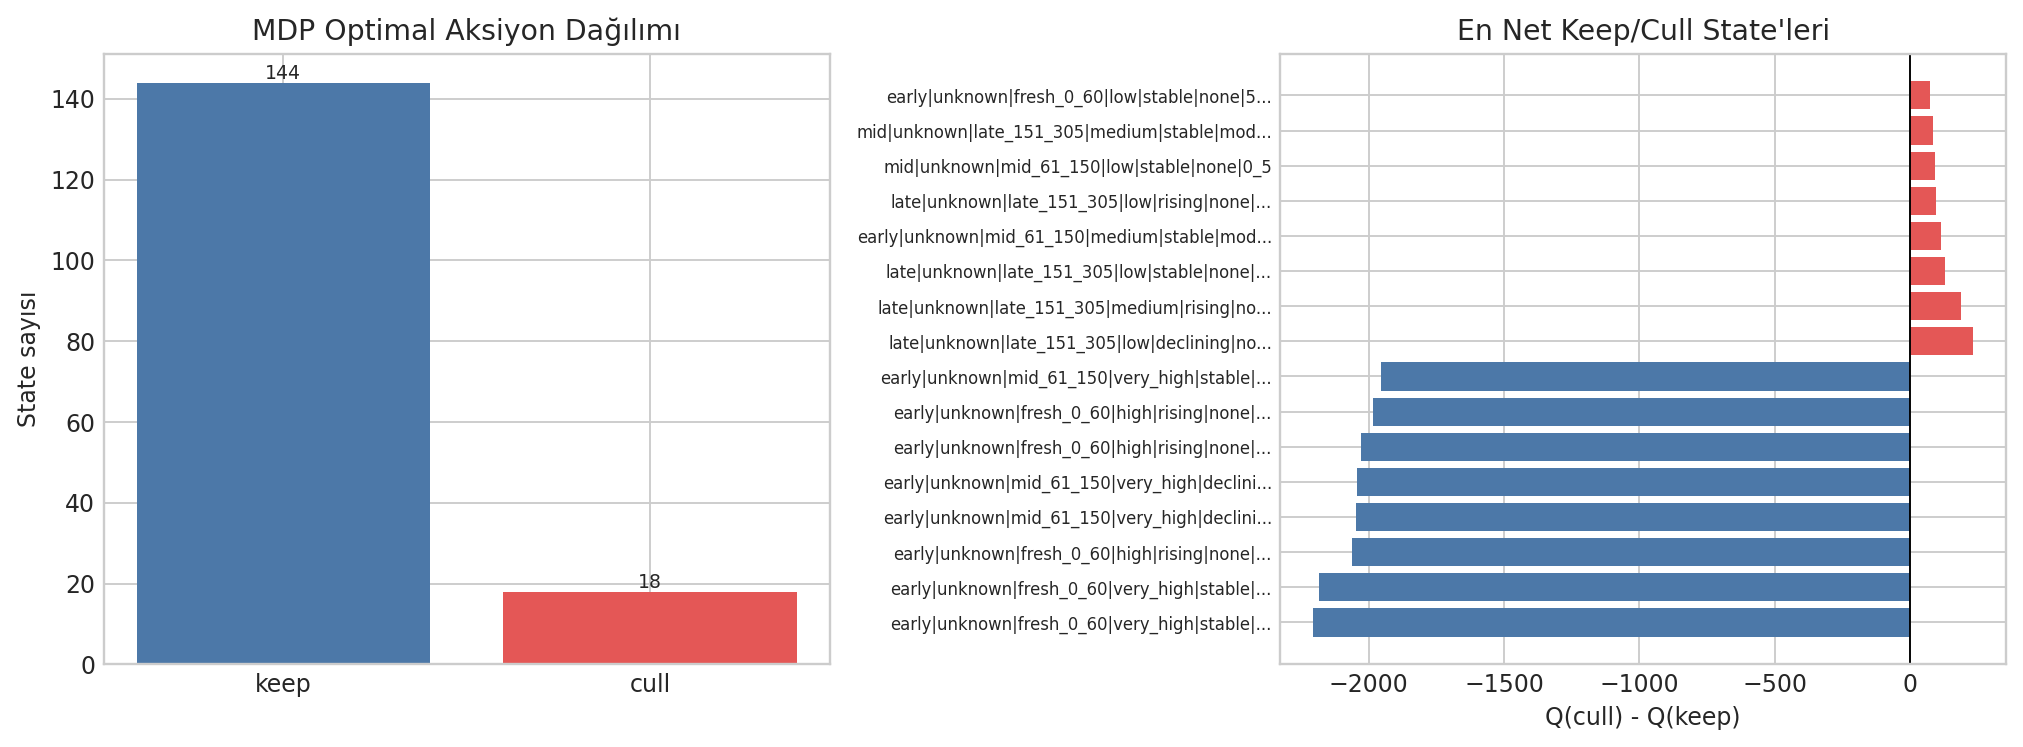
\includegraphics[width=\textwidth]{03_mdp_policy_distribution_and_margin.png}
\caption{MDP optimal aksiyon dağılımı ve en belirgin keep/cull karar marjları.}
\label{fig:mdp_policy_margin}
\end{figure*}

Şekil~\ref{fig:mdp_risk_band}, culling risk bandı ile MDP'nin cull eğilimi
arasındaki ilişkiyi özetler. Beklendiği gibi yüksek risk bantlarında cull
olasılığı artar; ancak karar basit bir risk threshold değildir. Aynı risk
bandındaki state'lerde süt seviyesi, süt trendi, sağlık riski, state desteği ve
transition fallback durumu policy sonucunu değiştirebilir. Bu, denetimli risk
modelinin nihai karar değil, MDP state girdisi olarak kullanılmasının doğru bir
tercih olduğunu gösterir.

\begin{figure*}[!t]
\centering
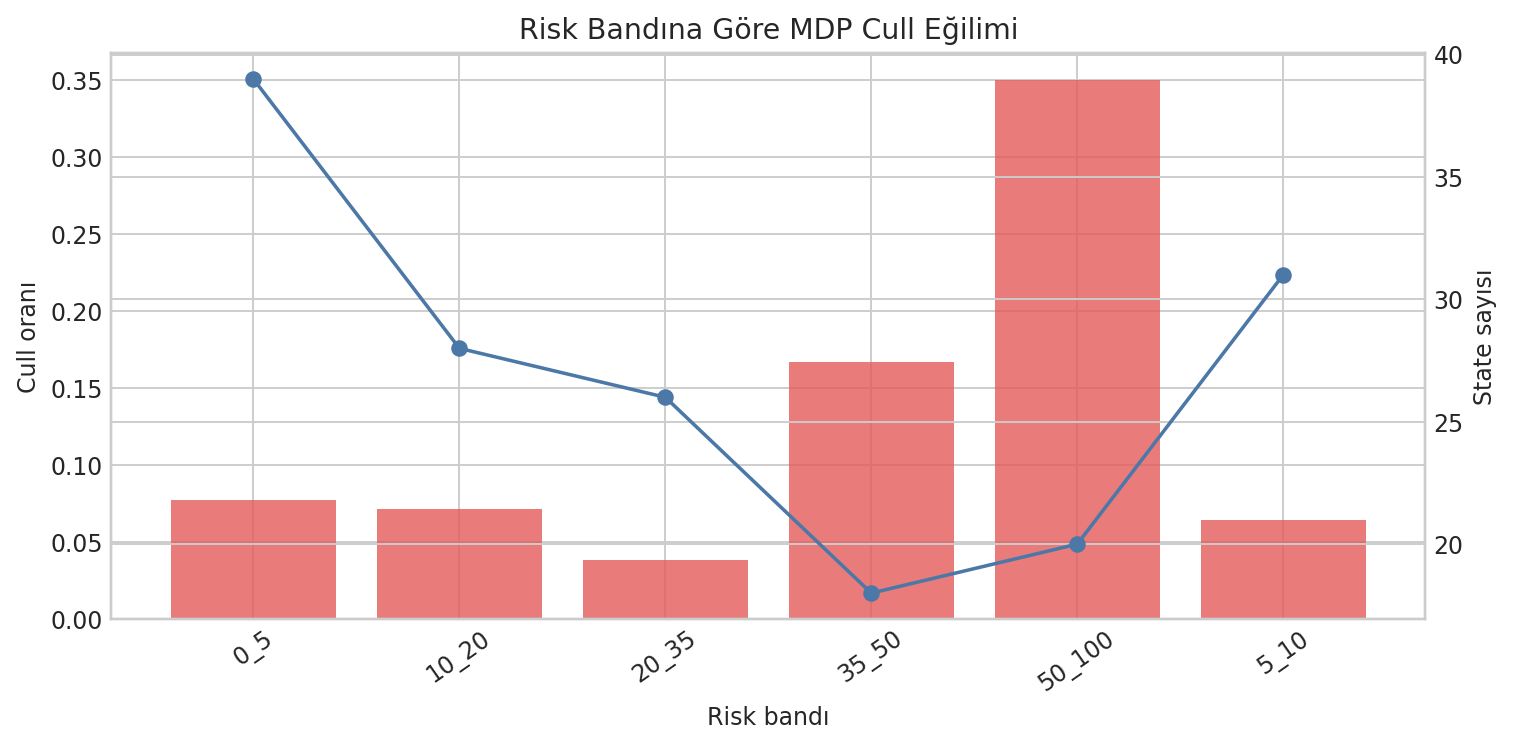
\includegraphics[width=0.92\textwidth]{04_mdp_cull_rate_by_risk_band.png}
\caption{Risk bandına göre MDP cull oranı ve state desteği.}
\label{fig:mdp_risk_band}
\end{figure*}

\subsection{Senaryo Hassasiyeti}
Senaryo analizi, reward varsayımlarının policy üzerinde belirgin etkisi
olduğunu göstermektedir. Örneğin süt fiyatının yüzde 20 artması cull durum
sayısını sıfıra indirirken, süt fiyatının yüzde 20 azalması cull durum sayısını
78'e yükseltmektedir. Bu sonuç beklenen bir davranıştır: replacement policy
ekonomik koşullara duyarlı olmalıdır. Aynı zamanda reward kalibrasyonunun
gerçek kullanım öncesinde çiftlik ve pazar özelinde yapılması gerektiğini
gösterir.

\begin{table}[!t]
\caption{Seçilmiş MDP Senaryo Hassasiyeti Sonuçları}
\label{tab:scenario}
\centering
\footnotesize
\setlength{\tabcolsep}{3pt}
\begin{tabular}{p{0.42\columnwidth}rrr}
\toprule
Senaryo & Keep & Cull & Değişen \\
\midrule
Baseline & 144 & 18 & 0 \\
Yüksek süt fiyatı & 162 & 0 & 18 \\
Düşük süt fiyatı & 84 & 78 & 60 \\
Yüksek replacement maliyeti & 150 & 12 & 6 \\
Düşük replacement maliyeti & 138 & 24 & 6 \\
Yüksek discount & 134 & 28 & 10 \\
\bottomrule
\end{tabular}
\end{table}

Şekil~\ref{fig:scenario_sensitivity}, senaryo etkisini üç açıdan gösterir:
cull state sayısı, baseline'a göre değişen state sayısı ve ortalama state
değeri. En güçlü etki süt fiyatında görülmektedir. Yüksek süt fiyatı keep
aksiyonunu ekonomik olarak daha değerli yaptığı için cull state sayısını sıfıra
indirir. Düşük süt fiyatı ise süt gelirini zayıflattığı için 78 state'i cull
kararına taşır. Replacement maliyeti değişimi daha sınırlı bir etki üretmiştir;
bu, mevcut reward ayarlarında süt gelirinin policy üzerinde replacement
maliyetinden daha baskın olduğunu gösterir. Discount faktörünün artması bazı
yüksek riskli state'lerde gelecekteki risk maliyetini daha görünür hale getirdiği
için cull sayısını artırmıştır. Bu sonuçlar, üretim ortamına geçmeden önce
reward parametrelerinin çiftlik ve piyasa özelinde kalibre edilmesi gerektiğini
açık biçimde ortaya koyar.

\begin{figure*}[!t]
\centering
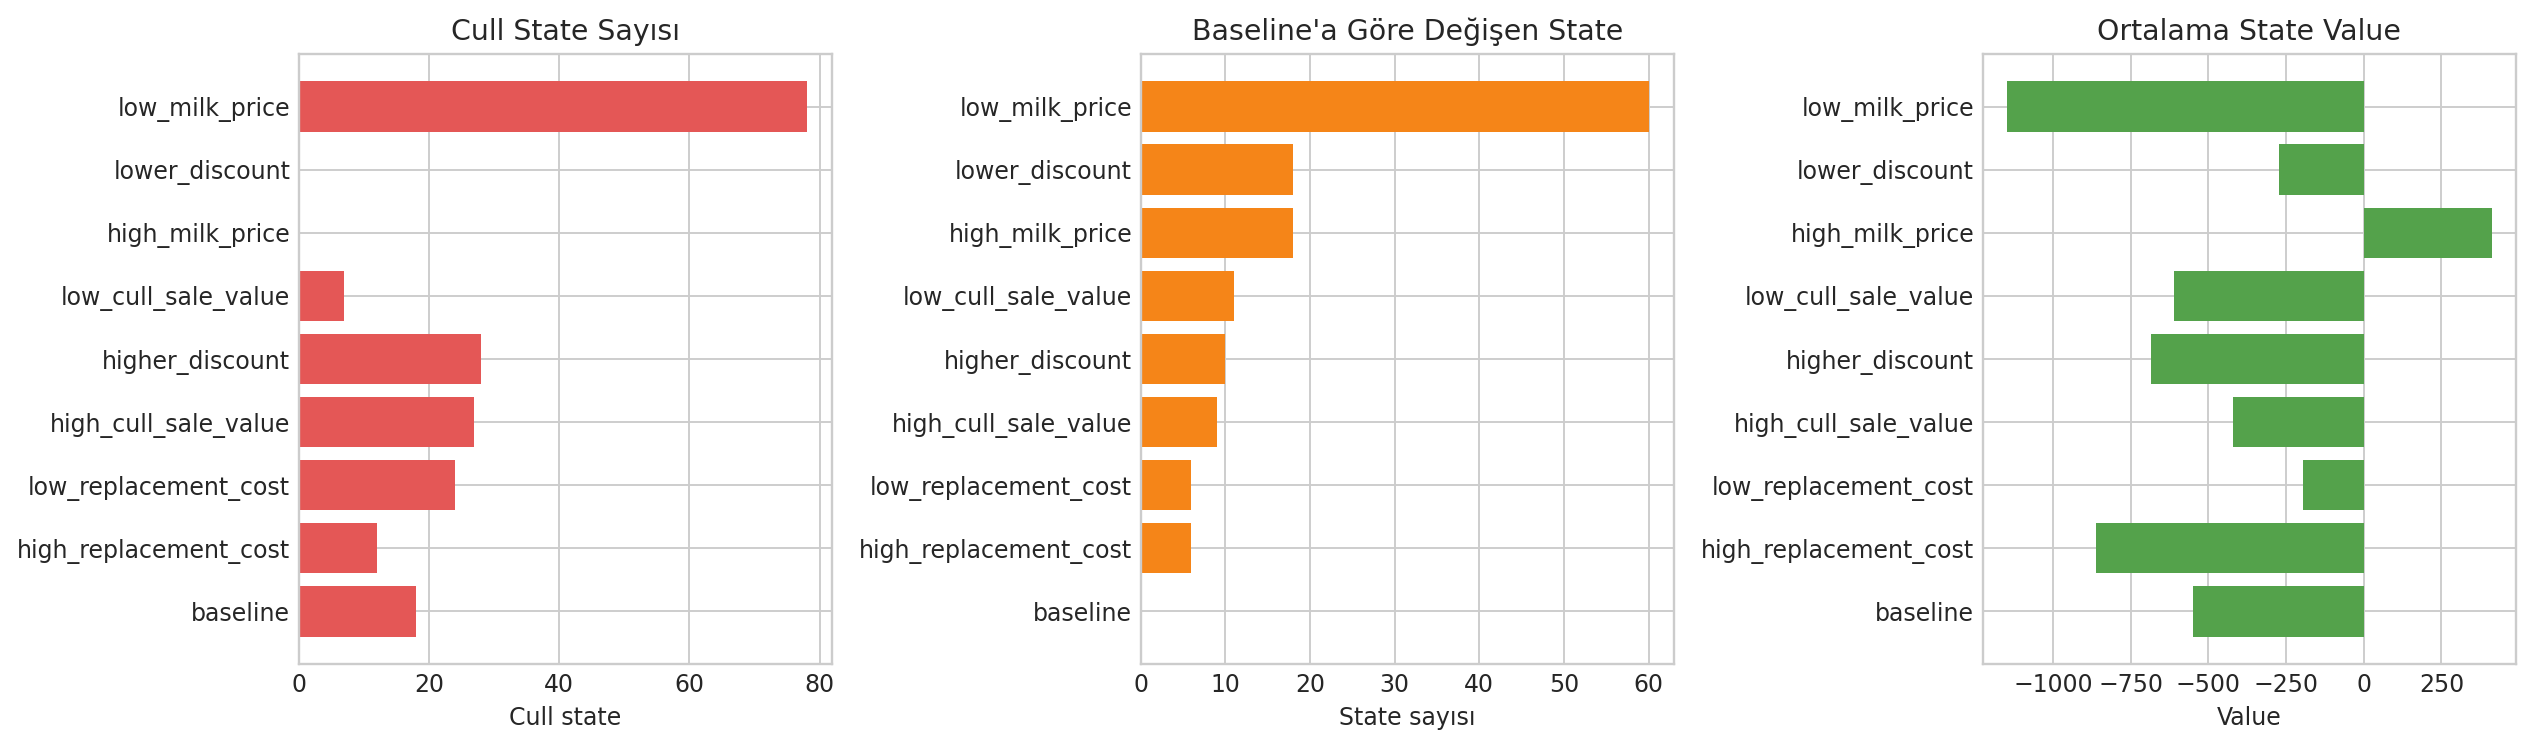
\includegraphics[width=\textwidth]{05_scenario_sensitivity.png}
\caption{Reward ve discount senaryolarına göre MDP policy hassasiyeti.}
\label{fig:scenario_sensitivity}
\end{figure*}

\subsection{RL Benchmark Sonuçları}
Model tabanlı value-iteration policy, tamamlanan benchmark satırları içinde en
iyi ortalama başlangıç değerini üretmiştir. Tabular Q-learning daha agresif bir
culling policy öğrenirken, DQN-style fitted Q MLP değerlendirilen konfigürasyonda
keep-all davranışına yakınsamıştır. Bu sonuçlar bu fazda model tabanlı MDP'nin
referans yöntem olarak kalmasını destekler.

\begin{table*}[!t]
\caption{Policy Benchmark Sonuçları}
\label{tab:rl_benchmarks}
\centering
\footnotesize
\begin{tabular}{lrrrr}
\toprule
Algoritma & Ortalama Başlangıç Değeri & Ortalama Durum Değeri & Cull Oranı & MDP'den Farklı \\
\midrule
Model tabanlı value iteration & -30.30 & -550.68 & 0.1111 & 0 \\
Keep all & -70.99 & -618.00 & 0.0000 & 18 \\
DQN-style fitted Q MLP & -70.99 & -618.00 & 0.0000 & 18 \\
Milk-margin threshold & -74.67 & -624.30 & 0.1235 & 20 \\
Tabular Q-learning & -93.10 & -739.24 & 0.1605 & 36 \\
Risk threshold & -164.90 & -732.55 & 0.2346 & 36 \\
Random policy & -622.02 & -909.79 & 0.0500 & 18 \\
Tabular PPO-style smoke & -1052.95 & -1195.45 & 0.4905 & 47 \\
Cull all now & -1300.00 & -1300.00 & 1.0000 & 144 \\
\bottomrule
\end{tabular}
\end{table*}

Şekil~\ref{fig:rl_algorithm_comparison}, algoritmaları iki eksende karşılaştırır:
ortalama başlangıç state değeri ve cull state oranı. Model tabanlı value
iteration en iyi ortalama başlangıç değerini üretir. Keep-all ve DQN-style
fitted Q MLP birbirine eşit görünmektedir; bu, MLP tabanlı fitted Q koşusunun bu
konfigürasyonda cull aksiyonunu yeterince öğrenemediğini ve güvenli tarafta
keep-all davranışına yakınsadığını gösterir. Tabular Q-learning ve risk
threshold daha yüksek cull oranı üretir; ancak bu agresiflik ortalama değeri
iyileştirmemiştir. Tabular PPO-style smoke test ise yaklaşık yarı state'te cull
seçerek aşırı agresif davranmış ve değer açısından zayıf kalmıştır. Bu tablo ve
grafik birlikte değerlendirildiğinde, bu fazda ana policy olarak model tabanlı
MDP'nin tutulması; tabular/approximate RL çıktılarının ise benchmark ve
validasyon sinyali olarak yorumlanması gerekir.

\begin{figure*}[!t]
\centering
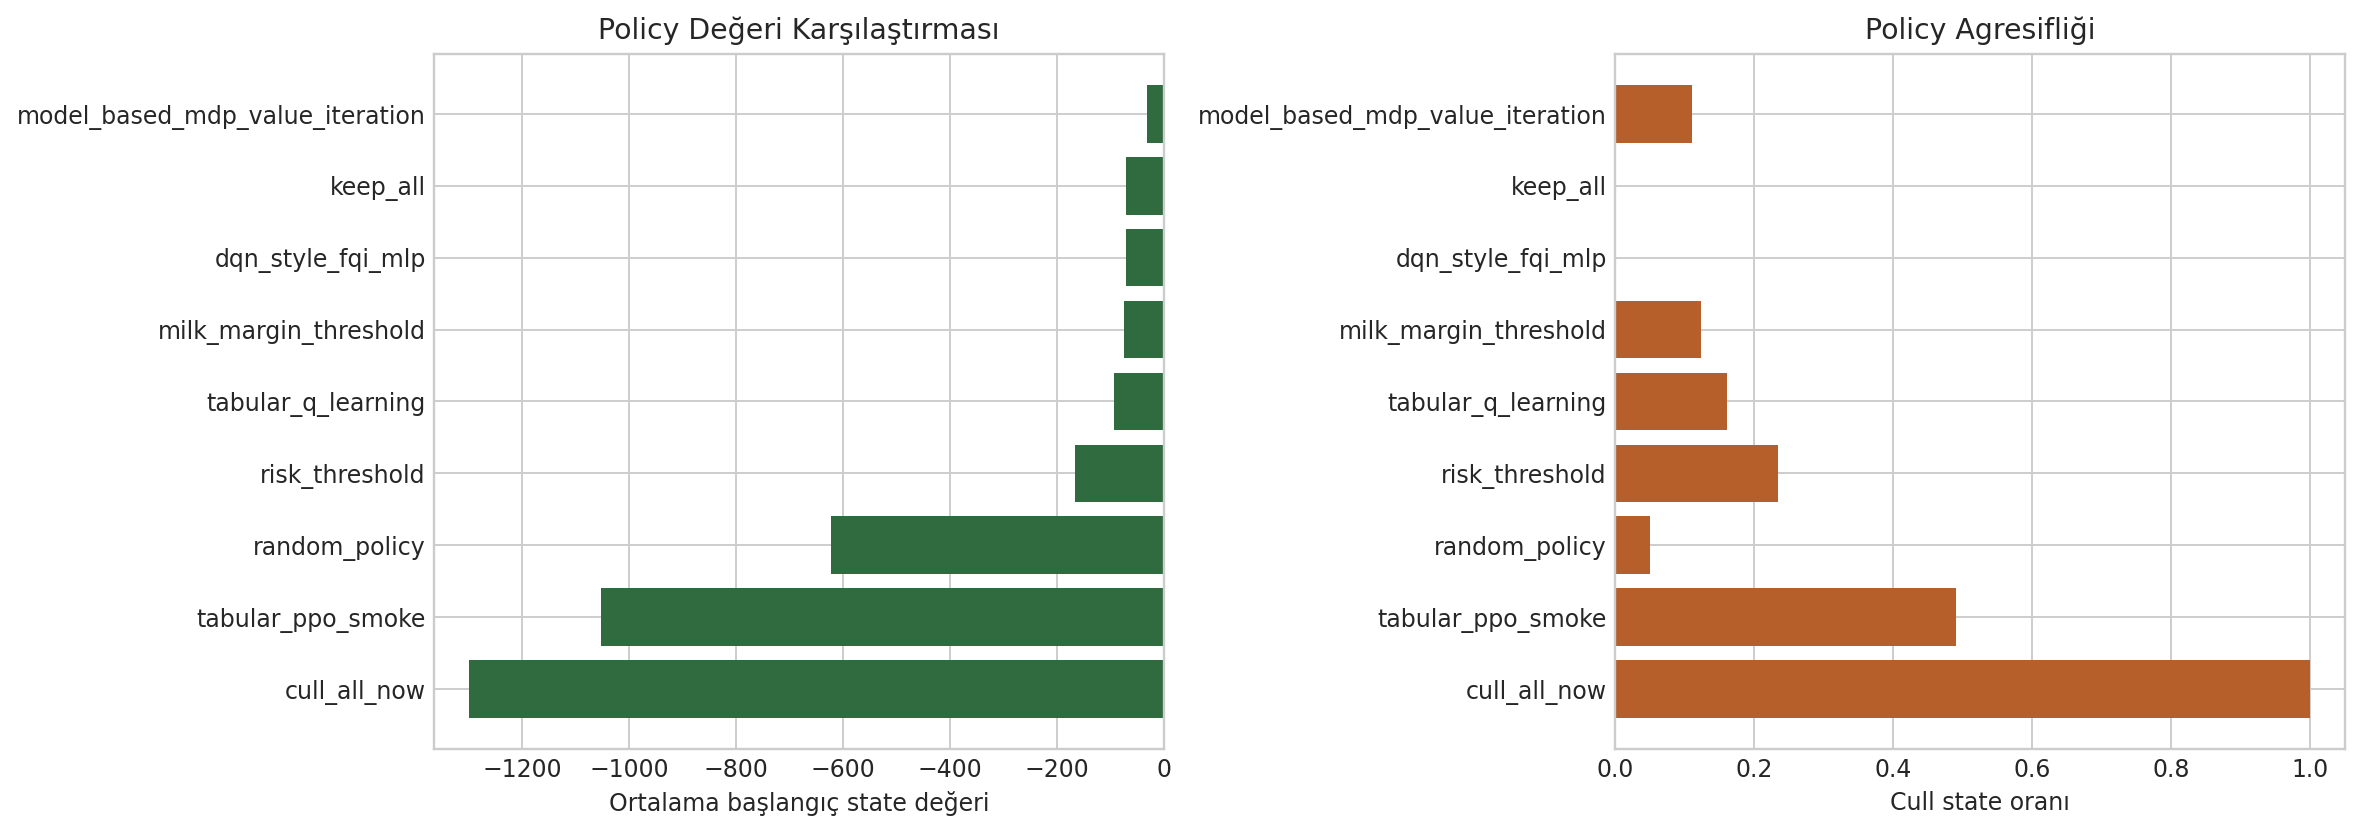
\includegraphics[width=\textwidth]{02_rl_algorithm_value_and_cull_rate.png}
\caption{RL/MDP algoritmalarının değer ve cull oranı karşılaştırması.}
\label{fig:rl_algorithm_comparison}
\end{figure*}

\subsection{Stable-Baselines3 DRL Sonuçları}
PPO ve DQN, ampirik Gymnasium simülatörü üzerinde 5.000 timestep boyunca
eğitilmiştir. Bu kısa eğitim koşusunda PPO, DQN'e göre daha yüksek ortalama
episode reward üretmiş ve durumların yüzde 14,81'inde cull seçmiştir. DQN ise
değerlendirilen konfigürasyonda tüm durumlarda keep seçmiştir.

\begin{table}[!t]
\caption{Stable-Baselines3 DRL Smoke Sonuçları}
\label{tab:sb3}
\centering
\footnotesize
\setlength{\tabcolsep}{3pt}
\begin{tabular}{p{0.14\columnwidth}rrrr}
\toprule
Model & Timestep & Ortalama Reward & Ortalama Adım & Cull Oranı \\
\midrule
PPO & 5.000 & -145.58 & 32.02 & 0.1481 \\
DQN & 5.000 & -401.86 & 33.48 & 0.0000 \\
\bottomrule
\end{tabular}
\end{table}

Şekil~\ref{fig:sb3_eval_summary}, PPO ve DQN'in kısa DRL koşularını özetler.
PPO, DQN'e göre daha yüksek ortalama reward üretmiş ve MDP'nin cull oranına
daha yakın bir aksiyon dağılımı göstermiştir. DQN'in cull oranı sıfırdır; bu
durum, kısa eğitim bütçesi ve seyrek/negatif terminal reward altında DQN'in
keep-all benzeri bir politikaya sıkıştığını düşündürür. Bu sonuç DQN'in
kullanılamaz olduğu anlamına gelmez; ancak mevcut simülatör ve hiperparametre
ayarlarıyla DQN'in production policy adayı olarak yorumlanmaması gerektiğini
gösterir.

\begin{figure*}[!t]
\centering
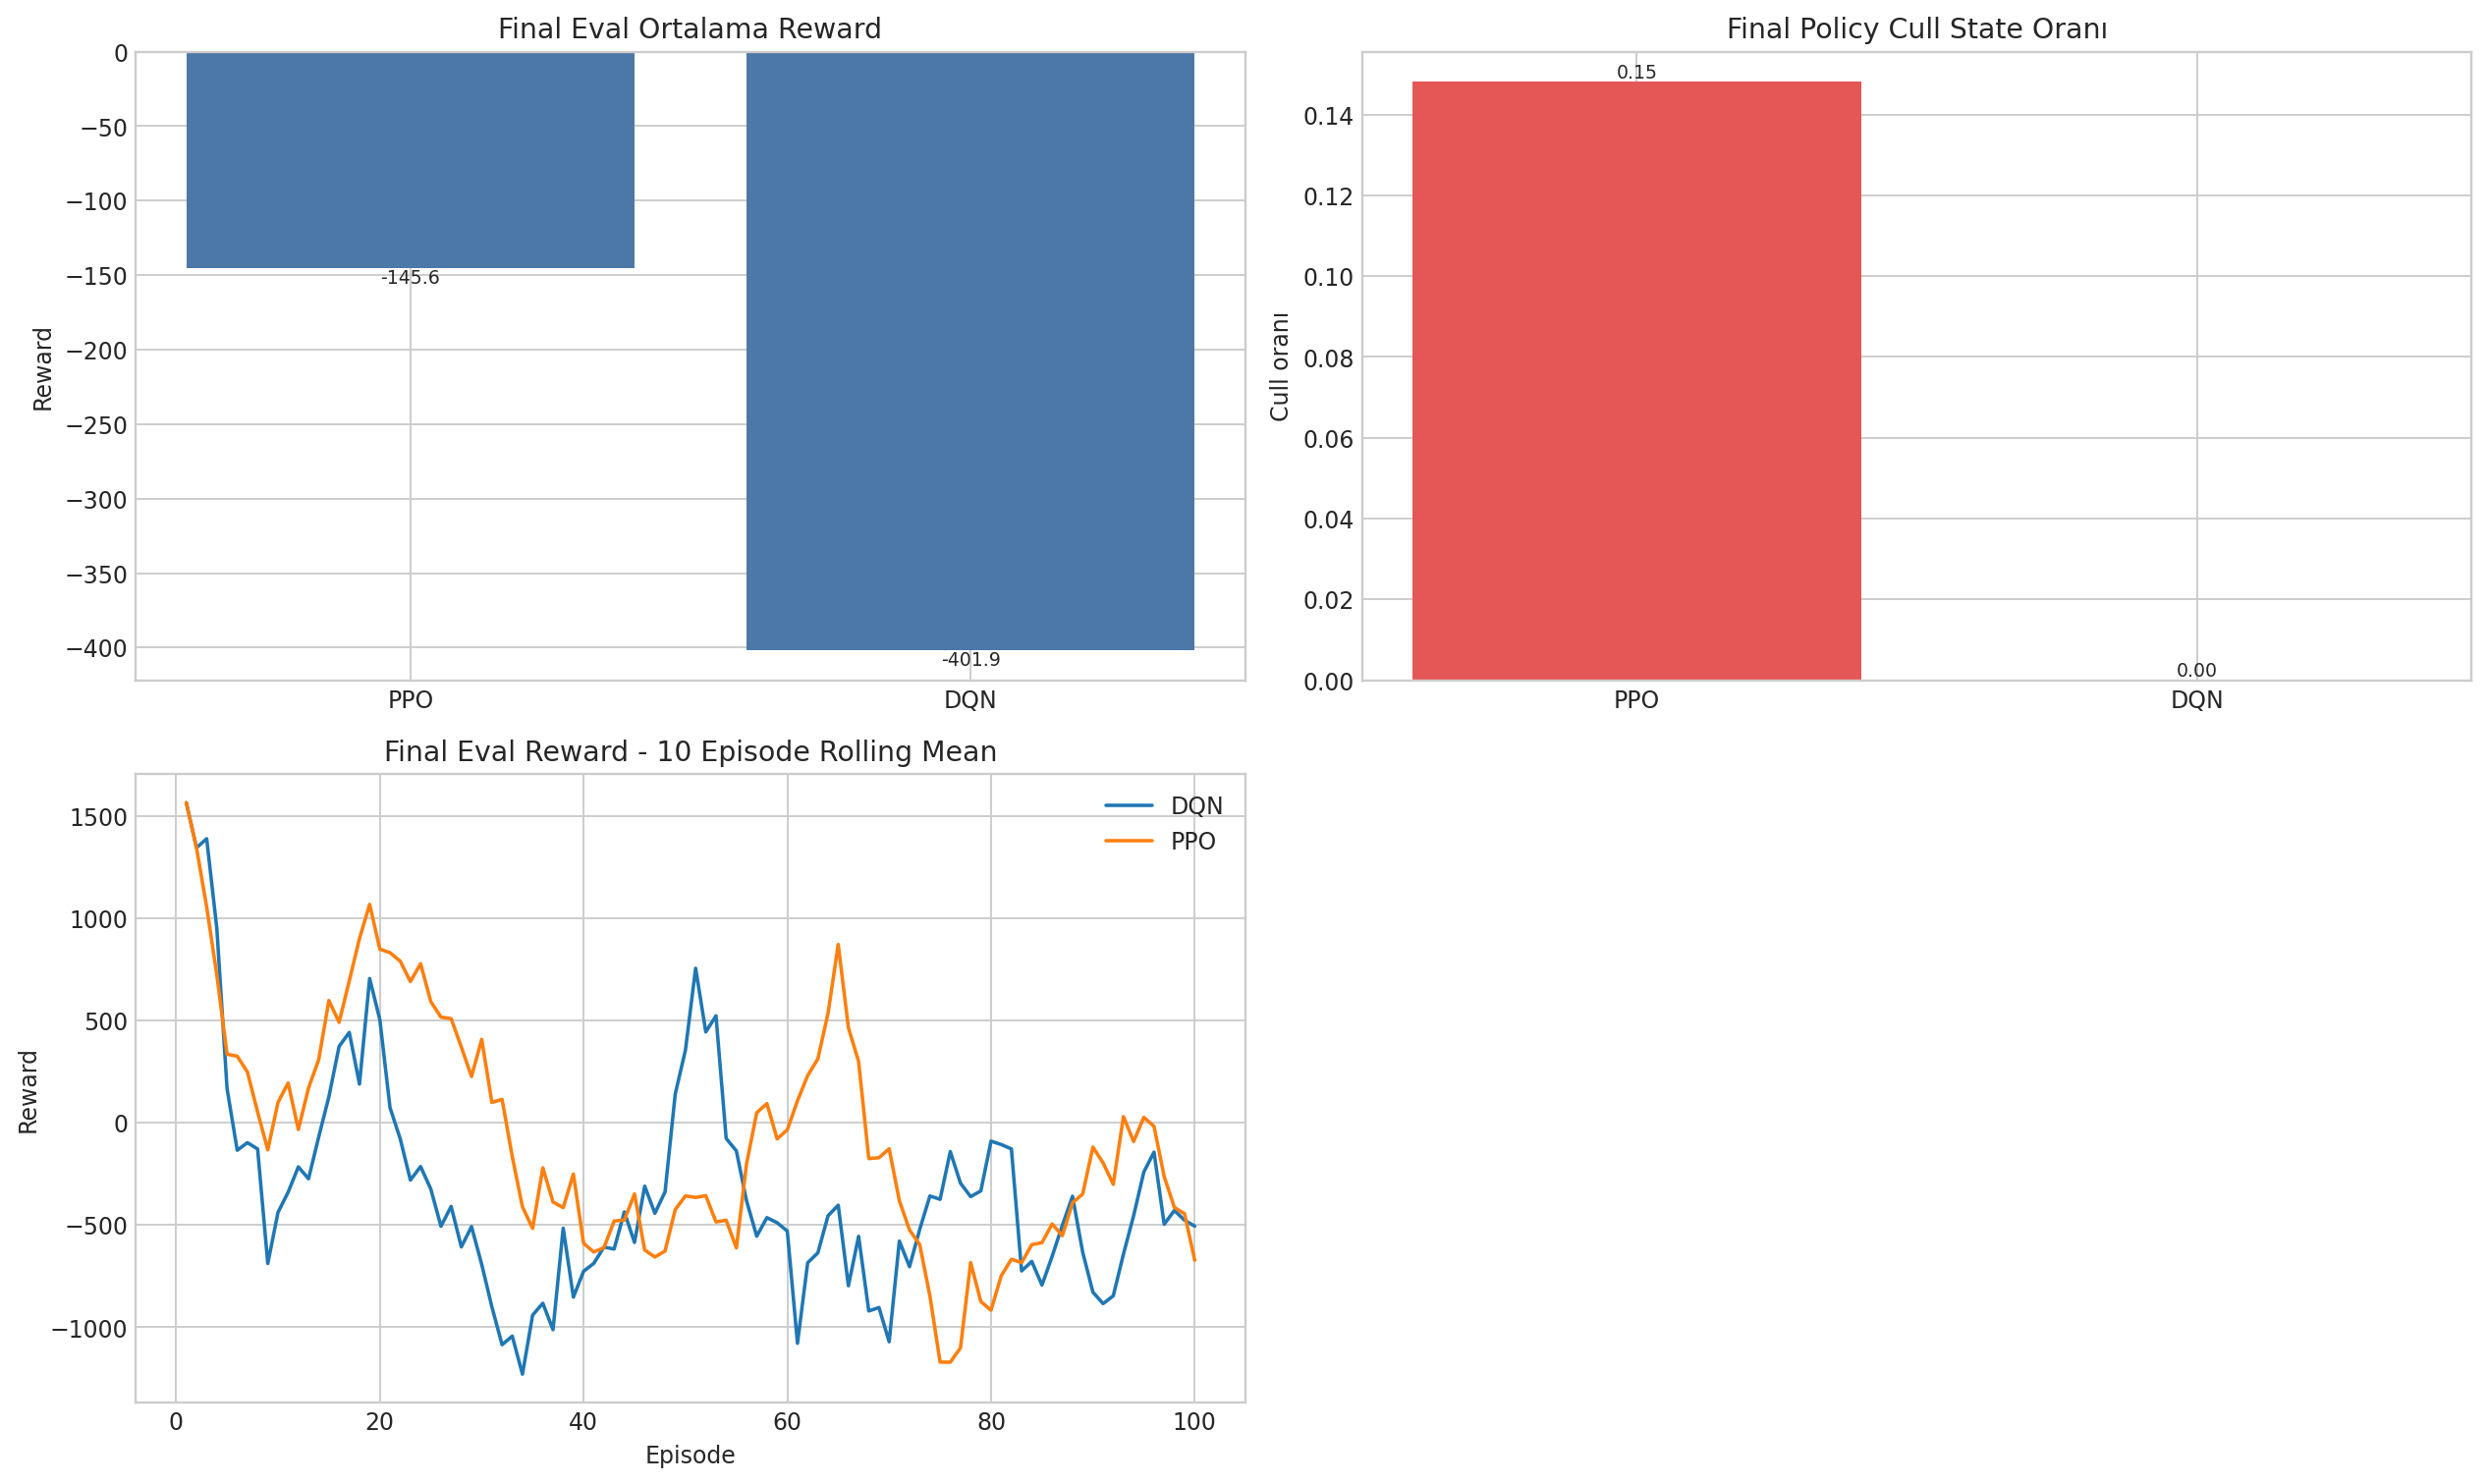
\includegraphics[width=\textwidth]{06_sb3_eval_summary.png}
\caption{Stable-Baselines3 PPO/DQN eval reward, cull oranı ve episode eğilimi.}
\label{fig:sb3_eval_summary}
\end{figure*}

Şekil~\ref{fig:sb3_reward_distribution}, episode reward dağılımını gösterir.
Dağılımın geniş olması, simülatörde başlangıç state'i ve rastlantısal geçişlerin
sonuç üzerinde belirgin etkisi olduğunu gösterir. PPO'nun ortalaması DQN'den
daha iyi olsa da varyansın yüksek olması, tek bir kısa DRL koşusundan nihai
karar çıkarmanın riskli olduğunu gösterir. Uzun eğitim, çoklu seed, senaryo
bazlı eval ve reward kalibrasyonu yapılmadan PPO/DQN çıktıları yalnızca
benchmark olarak kalmalıdır.

\begin{figure}[!t]
\centering
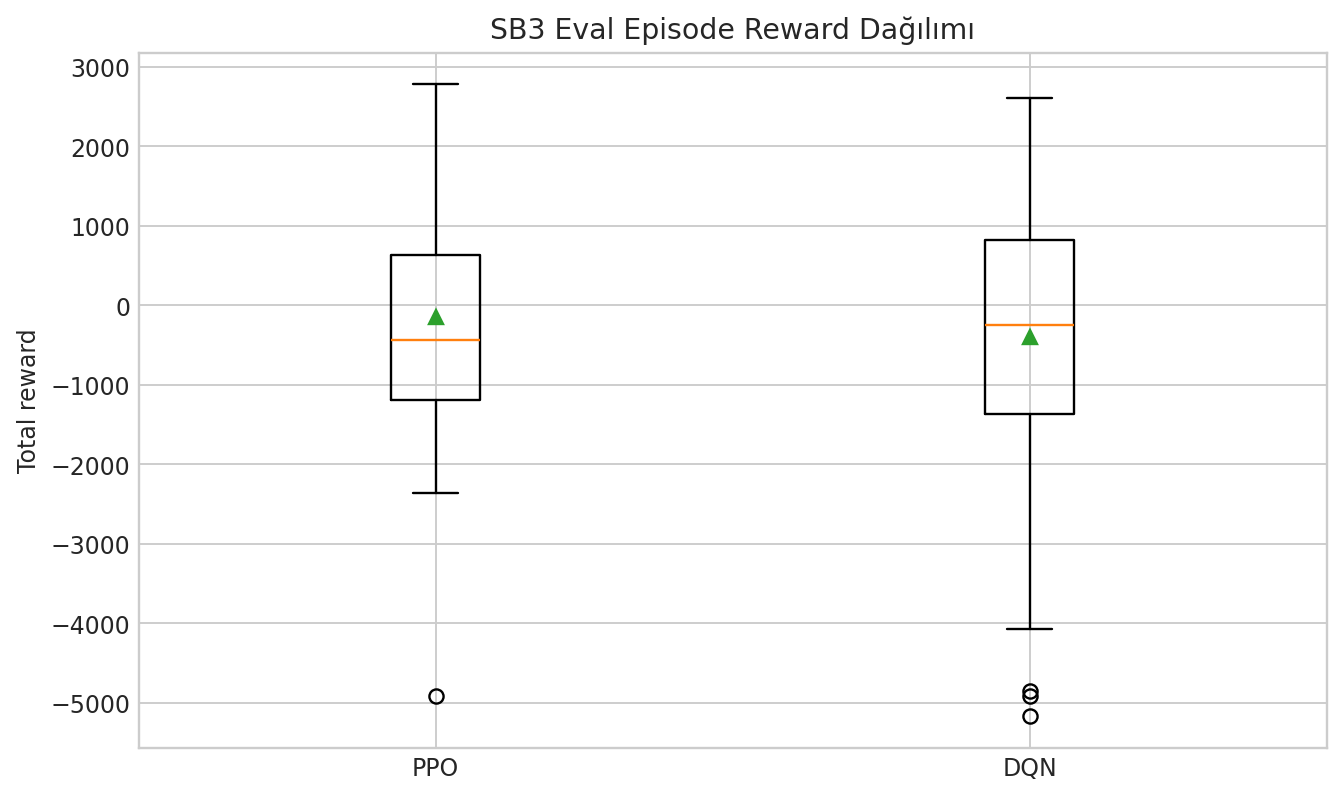
\includegraphics[width=\columnwidth]{07_sb3_eval_reward_distribution.png}
\caption{SB3 PPO/DQN eval episode reward dağılımı.}
\label{fig:sb3_reward_distribution}
\end{figure}

\subsection{Reward ve Simülasyon Davranışı}
Şekil~\ref{fig:reward_components}, keep ve cull reward dağılımlarını ve keep
aksiyonunun ortalama bileşenlerini gösterir. Cull reward'unun replacement
maliyeti nedeniyle güçlü biçimde negatif olması, policy'nin neden cull
aksiyonunu yalnızca belirli state'lerde seçtiğini açıklar. Keep tarafında süt
geliri ana pozitif bileşendir; bakım maliyeti ve beklenen culling riski maliyeti
ise ana negatif bileşenlerdir. Bu yapı biyolojik ve ekonomik olarak tutarlıdır:
yüksek süt geliri keep kararını desteklerken, yüksek risk ve düşük üretim cull
kararını daha olası hale getirir.

\begin{figure*}[!t]
\centering
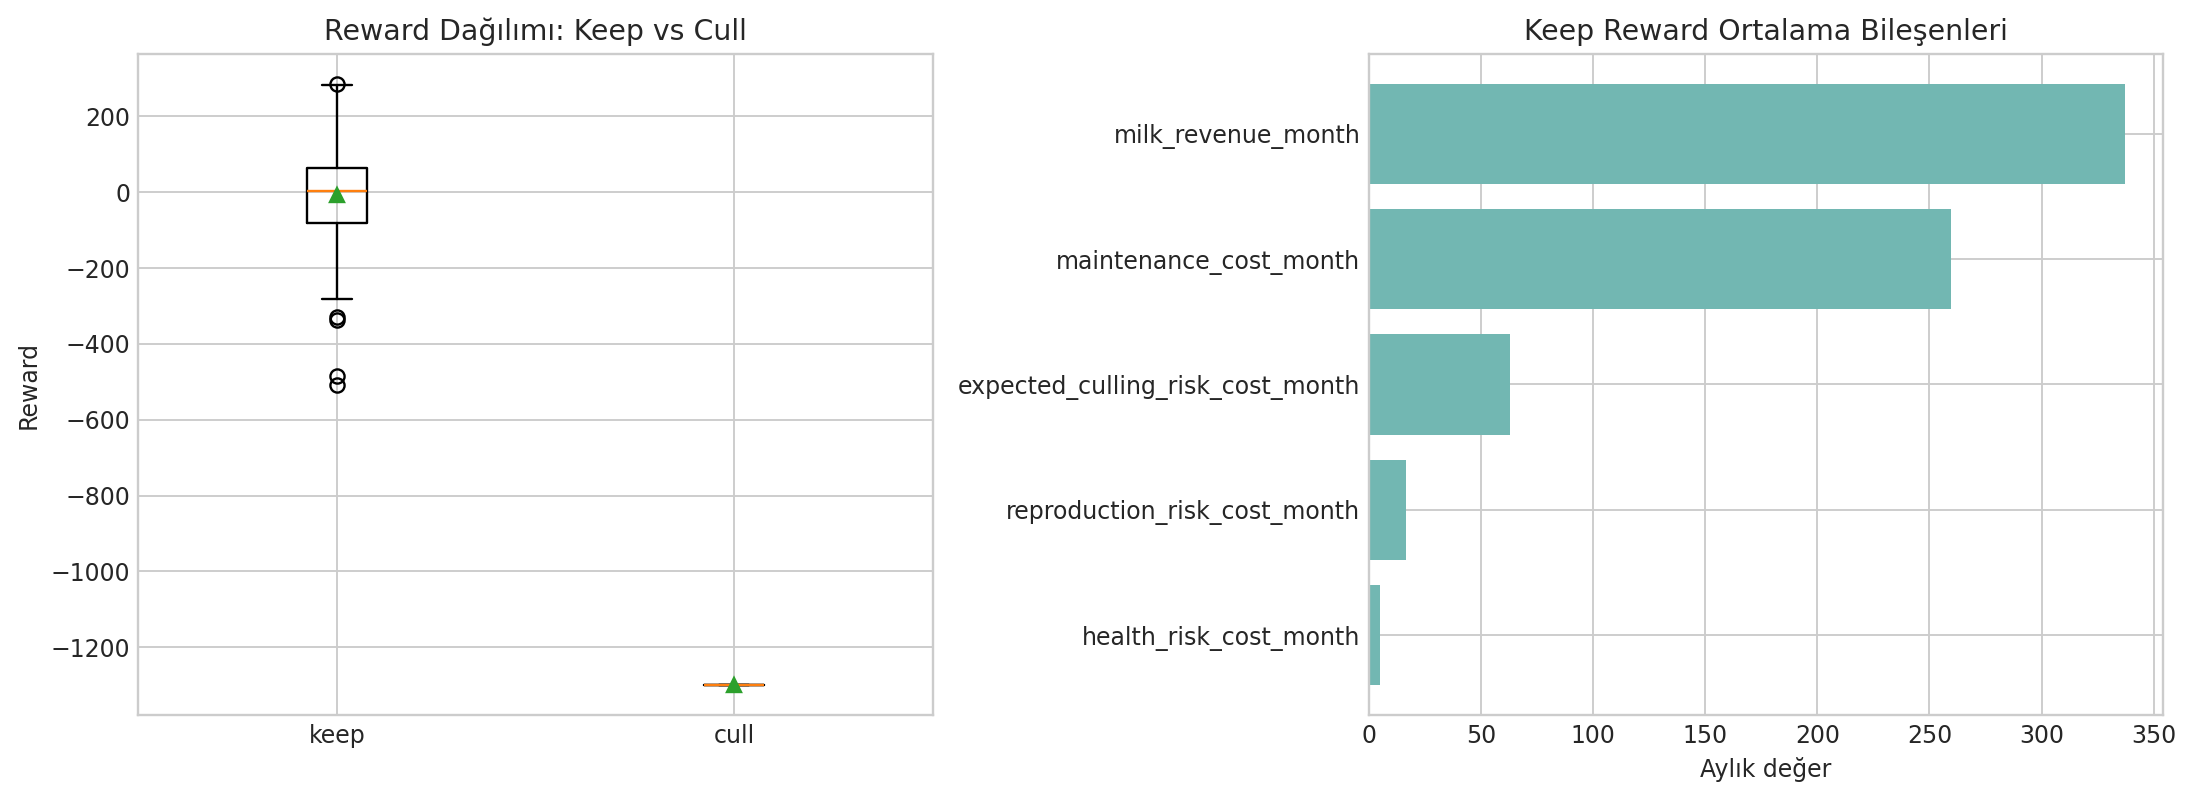
\includegraphics[width=\textwidth]{08_reward_distribution_and_components.png}
\caption{Reward dağılımı ve keep aksiyonu için ortalama ekonomik bileşenler.}
\label{fig:reward_components}
\end{figure*}

Şekil~\ref{fig:policy_simulation_summary}, rollout simülasyonunda heuristic
policy'lerin ortalama total reward ve terminal neden dağılımını karşılaştırır.
Risk-threshold policy bu simülasyon koşusunda keep-all'dan daha iyi ortalama
ödül üretmiştir; çünkü riskli state'lerde erken cull kararı alarak bazı uzun
vadeli negatif reward birikimini keser. Ancak Tablo~\ref{tab:rl_benchmarks}'te
görüldüğü gibi policy evaluation açısından model tabanlı MDP hala daha iyi
başlangıç değerine sahiptir. Bu fark önemlidir: kısa rollout simülasyonu ve
tam MDP policy evaluation aynı şeyi ölçmez. Rollout grafiği operasyonel davranış
farklarını gösterirken, value iteration tablosu tüm state uzayı üzerinde
Bellman tutarlı beklenen değeri temsil eder.

\begin{figure*}[!t]
\centering
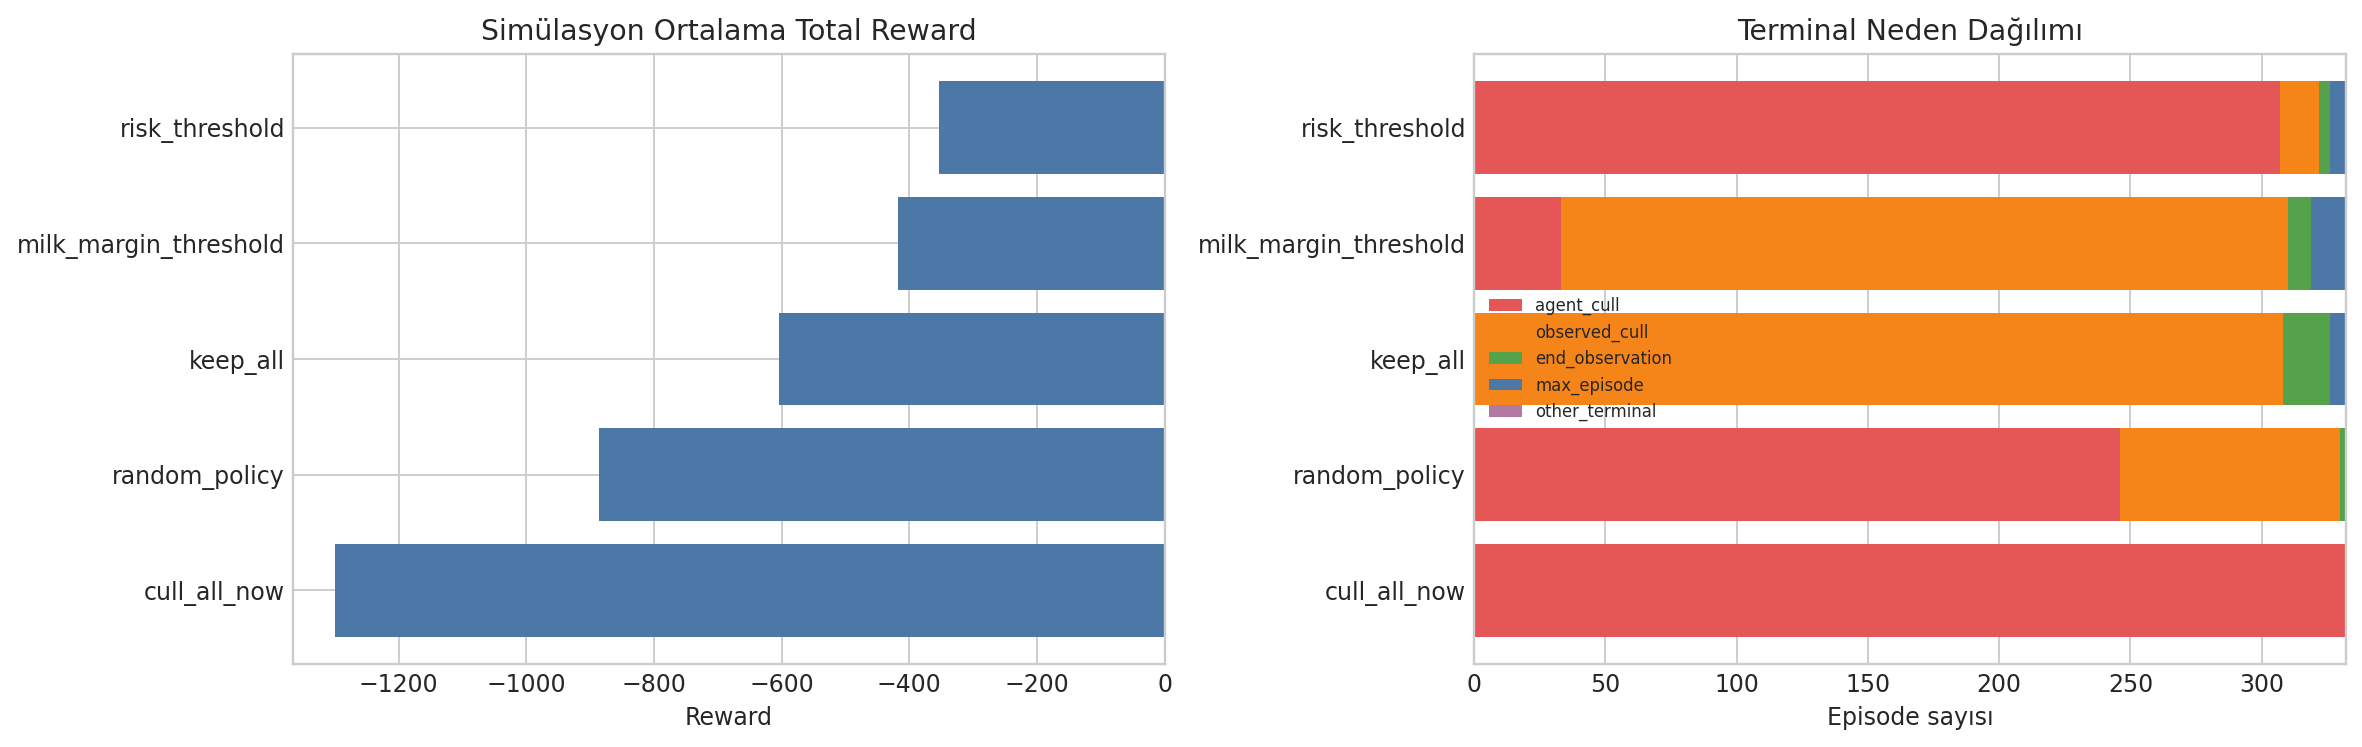
\includegraphics[width=\textwidth]{09_policy_simulation_summary.png}
\caption{Policy rollout simülasyonunda ortalama reward ve terminal neden dağılımı.}
\label{fig:policy_simulation_summary}
\end{figure*}

Şekil~\ref{fig:policy_trace_reward}, policy'lerin ay bazlı ortalama reward
eğilimini gösterir. Step ilerledikçe reward çizgilerinin ayrışması, keep/cull
kararının yalnızca ilk ay ödülünden değil, ardışık geçişlerden etkilendiğini
gösterir. Bu nedenle problem tek adımlı bir sınıflandırma veya sabit threshold
problemi olarak ele alınmamalıdır. MDP/RL katmanının değeri tam olarak burada
ortaya çıkar: aynı başlangıç riski farklı transition yollarında farklı ekonomik
sonuçlara ulaşabilir.

\begin{figure*}[!t]
\centering
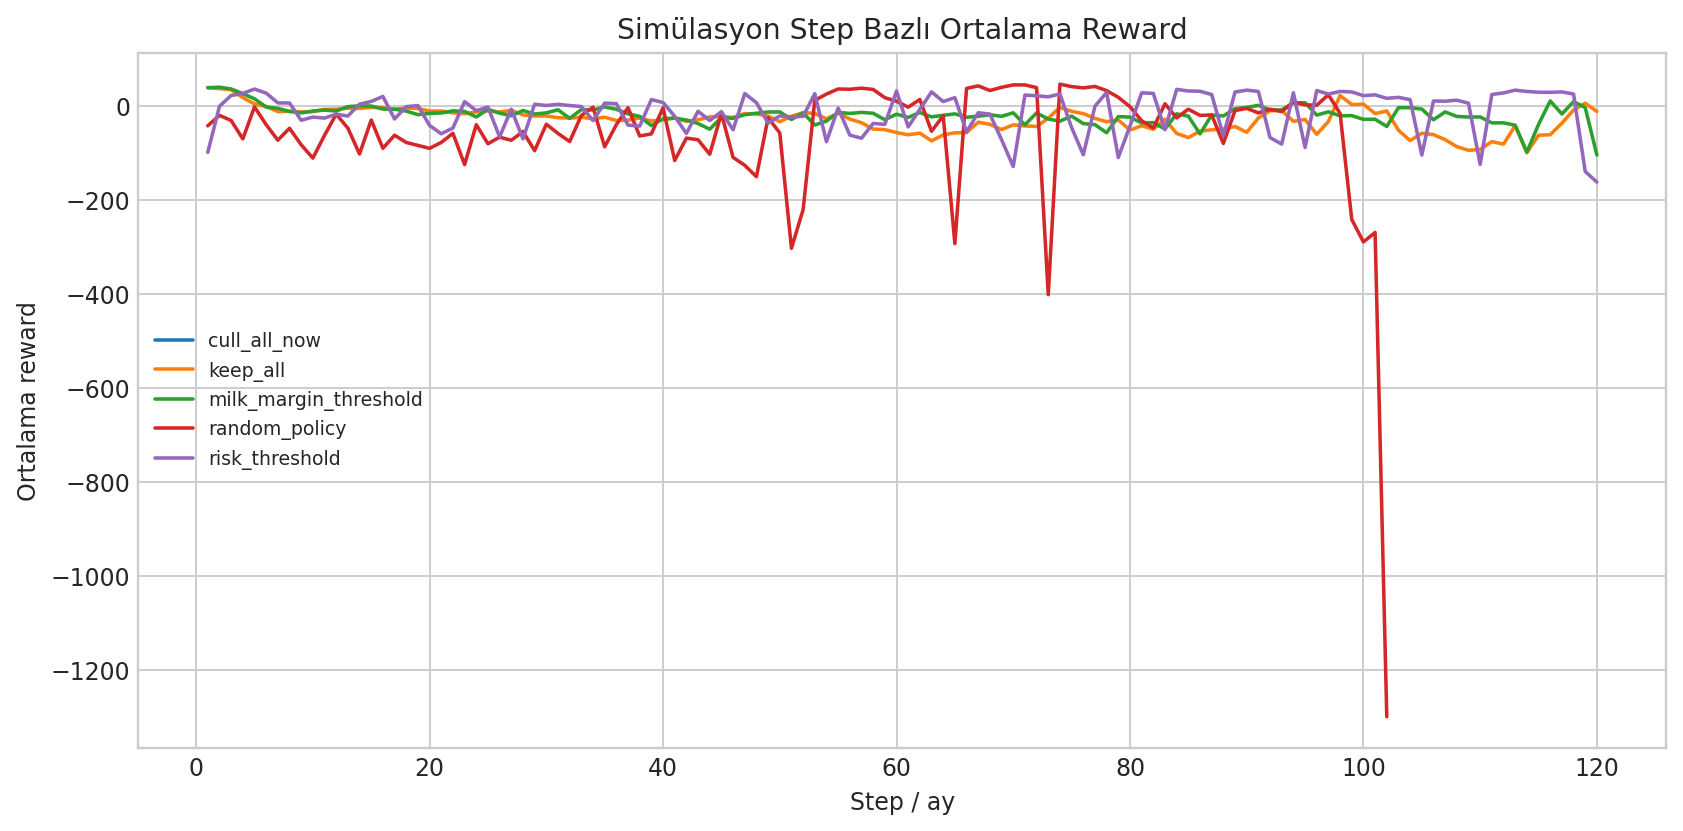
\includegraphics[width=\textwidth]{10_policy_trace_mean_reward_by_step.png}
\caption{Policy simülasyon trace'lerinde ay bazlı ortalama reward eğilimi.}
\label{fig:policy_trace_reward}
\end{figure*}

Genel sonuç olarak, bu deney setinde en güvenilir karar katmanı model tabanlı
MDP'dir. Supervised risk modeli MDP'ye anlamlı bir risk girdisi sağlar; ancak
nihai aksiyon risk threshold ile verilmemelidir. PPO kısa koşuda umut verici
bir DRL benchmark üretmiştir, fakat yüksek varyans ve simülatör kalibrasyonu
eksikliği nedeniyle ana policy değildir. DQN ve fitted Q koşuları ise mevcut
ayarlarla keep-all davranışına yakınsamış, bu da daha uzun eğitim, daha iyi
reward ölçekleme, replay/target ayarı ve çoklu seed validasyonu ihtiyacını
göstermiştir.

\section{Uygulama Yapısı}
RL kodu \path{Model/rl/code/} altında düzenlenmiştir. Merkezi eğitim ortamı ve
Gymnasium wrapper \path{training_environment.py} içinde yer alır. Model
implementasyonları ailelere ayrılmıştır: \path{models/model_based/},
\path{models/tabular/}, \path{models/approximate/},
\path{models/stable_baselines/} ve \path{models/offline/}. Registry katmanı tüm
çalıştırılabilir modelleri ortak \texttt{ModelRunSpec} arayüzü ile sunar.
Notebook runner parametre düzenleme, tek model çalıştırma, çoklu model
çalıştırma, output tablo inceleme, rapor önizleme ve run-manifest export
işlevlerini sağlar.

\section{Geçerlilik Tehditleri}
Tablo~\ref{tab:threats} prototipin akademik ve pratik yorumlanmasında dikkate
alınması gereken başlıca geçerlilik tehditlerini özetler.

\begin{table*}[!t]
\caption{Geçerlilik Tehditleri ve Etkileri}
\label{tab:threats}
\centering
\begin{tabular}{p{0.24\textwidth}p{0.36\textwidth}p{0.30\textwidth}}
\toprule
Tehdit & Açıklama & Azaltma Yaklaşımı \\
\midrule
Kaynak genellenebilirliği & Kamusal veri setleri hedef çiftlik popülasyonunu
tam temsil etmeyebilir. & Source-agnostic validasyon, farm-specific yeniden
kalibrasyon ve shadow-mode test. \\
Reward belirsizliği & Replacement, tedavi, bakım ve cull satış değerleri
çiftlik ve piyasa koşullarına bağlıdır. & Senaryo analizi ve çiftlik özelinde
ekonomik parametre kalibrasyonu. \\
Transition sparsity & Bazı ayrık state kovalarında geçiş desteği düşüktür. &
Fallback transition, learned transition modeli ve belirsizlik raporlaması. \\
Logged action eksikliği & Gerçek keep/cull karar aksiyonları aylık düzeyde
güvenilir değildir. & Offline RL'i ertelemek, davranış politikası veya gerçek
logged action toplamak. \\
Simulator bias & DRL modelleri gerçek çiftlik yerine prototip ampirik
simülatörde eğitilir. & Simülatör validasyonu, çoklu senaryo değerlendirme ve
uzman onay katmanı. \\
\bottomrule
\end{tabular}
\end{table*}

\section{Sınırlılıklar}
Bu prototipin önemli sınırlılıkları şunlardır:
\begin{itemize}
    \item Mevcut geçiş modeli ampirik ve ayrıklaştırılmıştır; seyrek durumlar
    fallback geçişlerine ihtiyaç duyar.
    \item Reward parametreleri karışık kaynaklı ve kısmen sentetiktir; hedef
    pazar ve çiftlik için kalibre edilmelidir.
    \item Denetimli risk etiketleri gözlemsel ve nadirdir; PR-AUC, ROC-AUC'ye
    göre daha bilgilendirici olsa da kaynak kompozisyonuna duyarlıdır.
    \item Gerçek logged keep/cull aksiyonları bulunmadığı için offline RL
    algoritmaları henüz geçerli değildir.
    \item SB3 PPO/DQN gerçek DRL koşularıdır; ancak doğrulanmış çiftlik
    simülatörü yerine prototip ampirik simülatör üzerinde eğitilmiştir.
\end{itemize}

\section{Gelecek Çalışmalar}
Bir sonraki teknik adımlar şunlardır:
\begin{enumerate}
    \item Süt fiyatı, yem maliyeti, replacement maliyeti, veteriner maliyeti ve
    cull satış değeri için çiftlik özelinde reward kalibrasyonu yapmak.
    \item Ayrık ampirik geçişleri learned transition modelleri ve belirsizlik
    tahminleri ile desteklemek veya değiştirmek.
    \item Öğrenilen tabular Q, fitted Q ve policy artifact'lerini metadata,
    seed, config hash ve veri hash bilgileriyle kalıcı hale getirmek.
    \item Ortam reset/step davranışı, reward hesabı, transition fallback ve
    value-iteration yakınsaması için unit test eklemek.
    \item CQL, IQL veya BCQ gibi offline RL yöntemleri denenmeden önce geçerli
    logged action verisi toplamak veya davranış politikası destekli simülasyon
    üretmek.
    \item DRL eğitimini daha uzun rollout, hiperparametre taraması ve çoklu
    reward senaryosu altında policy değerlendirmesi ile genişletmek.
\end{enumerate}

\section{Canlı Kullanıma Geçiş Yol Haritası}
Bu çalışma canlı karar sistemi değildir; ancak canlı kullanıma ilerlemek için
aşağıdaki kontrollü yol haritası izlenebilir:
\begin{enumerate}
    \item Çiftlik özelinde ekonomik parametrelerin ve biyolojik kısıtların
    uzmanlarla kalibre edilmesi.
    \item Gerçek keep/cull kararlarının, karar tarihi ve karar gerekçesiyle
    birlikte logged action olarak toplanması.
    \item MDP ve DRL policy çıktılarının yalnızca shadow-mode ortamda gerçek
    kararlarla karşılaştırılması.
    \item Veteriner, zooteknist ve işletme yöneticisi onayı içeren human-in-the-loop
    karar katmanının eklenmesi.
    \item Policy güvenlik sınırlarının tanımlanması; örneğin gebelik, sağlık
    tedavisi veya minimum gözlem desteği gibi durumlarda otomatik kararın
    devre dışı bırakılması.
    \item Pilot sürüde kontrollü A/B veya stepped-wedge deneme tasarımı ile
    ekonomik ve hayvan refahı etkilerinin ölçülmesi.
\end{enumerate}

\section{Sonuç}
Bu çalışma, süt sığırcılığında inek bazlı keep/cull karar desteği için uçtan
uca çevrimdışı bir prototip ortaya koymuştur. Mevcut en güçlü karar katmanı,
90 günlük denetimli culling-risk girdisi ve ampirik geçiş modeliyle desteklenen
model tabanlı MDP'nin value iteration ile çözülmüş halidir. Karşılaştırmalı RL
ve DRL deneyleri uygulanmış ve çalıştırılabilir hale getirilmiştir; ancak bu
sonuçlar simülatör, reward fonksiyonu ve logged-action veri katmanı
güçlendirilene kadar production policy değil araştırma benchmark'ı olarak
yorumlanmalıdır.

\section*{Teşekkür}
Bu rapor, LaktaSens karar destek prototipi kapsamında oluşturulan yerel
veri işleme, modelleme ve deney çıktıları esas alınarak hazırlanmıştır.

\renewcommand{\refname}{Kaynakça}
\begin{thebibliography}{00}

\bibitem{palma2025}
O. Palma, L. M. Plà-Aragonés, A. Mac Cawley, and V. M. Albornoz,
``Mathematical methods applied to the problem of dairy cow replacements: A
scoping review,'' \emph{Animals}, vol. 15, no. 7, Art. no. 970, 2025,
doi: 10.3390/ani15070970.

\bibitem{stewart1977}
H. M. Stewart, E. B. Burnside, J. W. Wilton, and W. C. Pfeiffer, ``A dynamic
programming approach to culling decisions in commercial dairy herds,''
\emph{Journal of Dairy Science}, vol. 60, no. 4, pp. 602--617, 1977,
doi: 10.3168/jds.S0022-0302(77)83908-8.

\bibitem{kristensen1987}
A. R. Kristensen, ``Optimal replacement and ranking of dairy cows determined by
a hierarchic Markov process,'' \emph{Livestock Production Science}, vol. 16,
no. 2, pp. 131--144, 1987, doi: 10.1016/0301-6226(87)90015-7.

\bibitem{delorenzo1992}
M. A. DeLorenzo, T. H. Spreen, G. R. Bryan, D. K. Beede, and J. A. M. van
Arendonk, ``Optimizing model: Insemination, replacement, seasonal production,
and cash flow,'' \emph{Journal of Dairy Science}, vol. 75, no. 3,
pp. 885--896, 1992, doi: 10.3168/jds.S0022-0302(92)77829-1.

\bibitem{yates1998}
C. M. Yates and T. Rehman, ``A linear programming formulation of the Markovian
decision process approach to modelling the dairy replacement problem,''
\emph{Agricultural Systems}, vol. 58, no. 2, pp. 185--201, 1998,
doi: 10.1016/S0308-521X(98)00054-7.

\bibitem{rajala2000}
P. J. Rajala-Schultz, Y. T. Gröhn, and H. G. Allore, ``Optimizing replacement
decisions for Finnish dairy herds,'' \emph{Acta Veterinaria Scandinavica},
vol. 41, no. 2, pp. 185--198, 2000, doi: 10.1186/BF03549650.

\bibitem{nielsen2010}
L. R. Nielsen, E. Jørgensen, A. R. Kristensen, and S. Østergaard, ``Optimal
replacement policies for dairy cows based on daily yield measurements,''
\emph{Journal of Dairy Science}, vol. 93, no. 1, pp. 75--92, 2010,
doi: 10.3168/jds.2009-2209.

\bibitem{shahinfar2014}
S. Shahinfar, A. S. Kalantari, V. E. Cabrera, and K. A. Weigel, ``Short
communication: Prediction of retention pay-off using a machine learning
algorithm,'' \emph{Journal of Dairy Science}, vol. 97, no. 5,
pp. 2949--2952, 2014, doi: 10.3168/jds.2013-7373.

\bibitem{adamczyk2021}
K. Adamczyk, W. Grzesiak, and D. Zaborski, ``The use of artificial neural
networks and a general discriminant analysis for predicting culling reasons in
Holstein-Friesian cows based on first-lactation performance records,''
\emph{Animals}, vol. 11, no. 3, Art. no. 721, 2021,
doi: 10.3390/ani11030721.

\bibitem{zhou2022}
X. Zhou, C. Xu, H. Wang, W. Xu, Z. Zhao, M. Chen, B. Jia, and B. Huang, ``The
early prediction of common disorders in dairy cows monitored by automatic
systems with machine learning algorithms,'' \emph{Animals}, vol. 12, no. 10,
Art. no. 1251, 2022, doi: 10.3390/ani12101251.

\bibitem{puterman1994}
M. L. Puterman, \emph{Markov Decision Processes: Discrete Stochastic Dynamic
Programming}. New York, NY, USA: Wiley, 1994.

\bibitem{sutton2018}
R. S. Sutton and A. G. Barto, \emph{Reinforcement Learning: An Introduction},
2nd ed. Cambridge, MA, USA: MIT Press, 2018.

\bibitem{mnih2015}
V. Mnih \emph{et al.}, ``Human-level control through deep reinforcement
learning,'' \emph{Nature}, vol. 518, pp. 529--533, 2015.

\bibitem{schulman2017}
J. Schulman, F. Wolski, P. Dhariwal, A. Radford, and O. Klimov, ``Proximal
policy optimization algorithms,'' arXiv:1707.06347, 2017.

\bibitem{kumar2020cql}
A. Kumar, A. Zhou, G. Tucker, and S. Levine, ``Conservative Q-learning for
offline reinforcement learning,'' in \emph{Proc. NeurIPS}, 2020.

\bibitem{kostrikov2021iql}
I. Kostrikov, A. Nair, and S. Levine, ``Offline reinforcement learning with
implicit Q-learning,'' arXiv:2110.06169, 2021.

\bibitem{fujimoto2019bcq}
S. Fujimoto, D. Meger, and D. Precup, ``Off-policy deep reinforcement learning
without exploration,'' in \emph{Proc. ICML}, 2019.

\bibitem{gymnasium}
M. Towers \emph{et al.}, ``Gymnasium: A standard interface for reinforcement
learning environments,'' arXiv:2407.17032, 2024.

\bibitem{stablebaselines3}
A. Raffin \emph{et al.}, ``Stable-Baselines3: Reliable reinforcement learning
implementations,'' \emph{Journal of Machine Learning Research}, vol. 22, no.
268, pp. 1--8, 2021.

\bibitem{projectreports}
LaktaSens KDS projesi, ``Suru keep/cull internal generated reports,'' proje
raporları dizini altında üretilen iç prototip raporları, 2026.

\bibitem{datasets}
LaktaSens KDS projesi, ``Dış veri kaynakları kataloğu ve dosya inceleme
raporları,'' \texttt{config/data\_sources.yaml} ve \texttt{reports/}
dizini altında üretilen proje içi veri kaynak dokümantasyonu, 2026.

\end{thebibliography}

\end{document}
